% ============================================================================
%  Báo cáo Bài tập lớn DSAI 261 - Dự báo nhu cầu điện năng theo giờ (Tây Ban Nha)
%  Biên dịch: mọi file sinh ra (aux, log, pdf, ...) nằm trong ../build
%   - VS Code (LaTeX Workshop): bấm Build, đã cấu hình outDir trong .vscode/settings.json
%   - Terminal: cd vào thư mục src rồi chạy `latexmk main.tex` (đọc file src/latexmkrc)
%  Hình ảnh lấy từ ../figures (copy từ energy-demand-forecasting/plots).
% ============================================================================
\documentclass[12pt,a4paper]{article}

\usepackage[utf8]{inputenc}
\usepackage[T5]{fontenc}
\usepackage[vietnamese]{babel}
\usepackage{lmodern}
\usepackage[a4paper,margin=2.3cm]{geometry}
\usepackage{amsmath,amssymb}
\usepackage{graphicx}
\usepackage{booktabs,tabularx,multirow,array,longtable}
\usepackage{float}
\usepackage{caption,subcaption}
\usepackage{xcolor}
\usepackage{listings}
\usepackage{enumitem}
\usepackage{fancyhdr}
\usepackage{siunitx}
\usepackage[hidelinks]{hyperref}
\usepackage{cleveref}
\crefname{table}{bảng}{bảng}\Crefname{table}{Bảng}{Bảng}
\crefname{figure}{hình}{hình}\Crefname{figure}{Hình}{Hình}
\crefname{section}{mục}{mục}\Crefname{section}{Mục}{Mục}
\crefname{subsection}{mục}{mục}\Crefname{subsection}{Mục}{Mục}
\crefname{subsubsection}{mục}{mục}\Crefname{subsubsection}{Mục}{Mục}
\crefname{equation}{công thức}{công thức}\Crefname{equation}{Công thức}{Công thức}
\crefname{listing}{đoạn mã}{đoạn mã}\Crefname{listing}{Đoạn mã}{Đoạn mã}
\crefname{lstlisting}{đoạn mã}{đoạn mã}\Crefname{lstlisting}{Đoạn mã}{Đoạn mã}
\crefname{appendix}{phụ lục}{phụ lục}\Crefname{appendix}{Phụ lục}{Phụ lục}

\graphicspath{{../figures/}{figures/}}
\sisetup{group-separator={,},group-minimum-digits=4}
\setlist{itemsep=2pt,topsep=4pt}

\definecolor{codebg}{RGB}{247,247,247}
\definecolor{codekw}{RGB}{0,0,160}
\definecolor{codecm}{RGB}{0,120,0}
\lstset{
  language=Python, basicstyle=\ttfamily\footnotesize, backgroundcolor=\color{codebg},
  keywordstyle=\color{codekw}\bfseries, commentstyle=\color{codecm}\itshape,
  stringstyle=\color{red!60!black}, frame=single, rulecolor=\color{gray!40},
  breaklines=true, showstringspaces=false, columns=fullflexible, numbers=left,
  numberstyle=\tiny\color{gray}, xleftmargin=1.5em, framexleftmargin=1.5em,
  literate={ŷ}{{$\hat{y}$}}1 {°}{{$^\circ$}}1
}

\newcommand{\todo}[1]{\noindent\colorbox{yellow!30}{\parbox{\dimexpr\linewidth-2\fboxsep}{\small\textbf{TODO:} #1}}}
\newcommand{\code}[1]{\texttt{\detokenize{#1}}}

\pagestyle{fancy}
\fancyhf{}
\lhead{\small DSAI 261 -- Dự báo nhu cầu điện năng}
\rhead{\small\thepage}
\renewcommand{\headrulewidth}{0.4pt}

\title{\textbf{Dự báo nhu cầu điện năng theo giờ tại Tây Ban Nha\\bằng các mô hình học máy}\\[4pt]
\large Bài tập lớn môn Khoa học dữ liệu \& Trí tuệ nhân tạo (DSAI) -- HK 261}
\author{Nhóm thực hiện: A, B, C, D, E}
\date{\today}

\begin{document}
\maketitle
\thispagestyle{empty}

\begin{abstract}
\noindent Báo cáo trình bày một hệ thống dự báo phụ tải điện (\emph{total load actual}) theo giờ cho
Tây Ban Nha giai đoạn 2015--2018, sử dụng bộ dữ liệu năng lượng của ENTSO-E kết hợp thời tiết của
5 thành phố lớn. Bài toán chính là \textbf{dự báo trước một ngày} (day-ahead, $h=24$ giờ). Phiên bản này
trình bày chi tiết hai phần: \textbf{(B)} xây dựng đặc trưng lịch, độ trễ và thời tiết không rò rỉ thông tin
tương lai cùng khung repo/báo cáo; \textbf{(C)} xây dựng mô-đun đánh giá dùng chung \code{evaluate.py},
các mô hình cơ sở, Ridge/Lasso và Random Forest. Trên tập kiểm tra (05--12/2018), Random Forest đạt
MAE 1\,530~MW (MAPE 5.22\%), giảm 39.6\% MAE so với mô hình ngây thơ $t-24$h và tốt hơn Ridge/Lasso
(MAPE 6.14\%). Phân tích ablation cho thấy tổ hợp đặc trưng lịch + độ trễ đóng góp phần lớn độ chính xác.
\end{abstract}

\tableofcontents
\newpage

% Người viết: A + E
\section{Giới thiệu}\label{sec:intro}
Dự báo phụ tải điện ngắn hạn (\emph{short-term load forecasting}, STLF) là đầu vào cho việc lập lịch
huy động nguồn, thị trường điện ngày tới (day-ahead market) và vận hành an toàn lưới điện. Sai số dự báo
chỉ 1\% cũng tương ứng với hàng trăm MW cần huy động dự phòng. Nhóm xây dựng một hệ thống dự báo phụ tải
toàn quốc của Tây Ban Nha theo giờ từ dữ liệu lịch sử phụ tải, lịch và thời tiết.

\paragraph{Phát biểu bài toán.} Gọi $y_t$ là phụ tải thực tế (MW) tại giờ $t$. Với chân trời dự báo
$h$ (mặc định $h=24$), cần học hàm $f$ sao cho
\begin{equation}
  \hat{y}_t = f\bigl(y_{t-h}, y_{t-h-1}, \dots;\ \text{lịch}_t;\ \text{thời tiết}_t\bigr),
\end{equation}
tức là chỉ được dùng các giá trị phụ tải đã quan sát được tại thời điểm phát hành dự báo $t-h$.

\todo{A + E bổ sung: động lực, mục tiêu, đóng góp chính, cấu trúc báo cáo.}

\section{Tổng quan tài liệu}\label{sec:lit}
\subsection{Dự báo phụ tải điện và các phương pháp truyền thống}\label{sec:lit-general}
% Người viết: E
Các hướng tiếp cận kinh điển gồm mô hình chuỗi thời gian (ARIMA/SARIMA), hồi quy tuyến tính có đặc trưng
lịch và nhiệt độ, và các mô hình học máy như Random Forest~\cite{breiman2001random}. Tổng quan của
Hong \& Fan~\cite{hong2016probabilistic} và cuộc thi GEFCom2014~\cite{hong2016gefcom} cho thấy các đặc trưng
lịch, độ trễ phụ tải và nhiệt độ là các yếu tố quyết định chất lượng dự báo.

\todo{E viết tiếp mục 2.1.}

\subsection{Các mô hình Gradient Boosting}\label{sec:lit-boosting}
% Người viết: D
\todo{D viết mục 2.2: Gradient Boosting, LightGBM, XGBoost.}

% Người viết: A
\section{Dữ liệu}\label{sec:data}
Bộ dữ liệu \emph{Hourly energy demand generation and weather}~\cite{kaggle_dataset} gồm hai bảng:
\code{energy_dataset.csv} (35\,064 giờ $\times$ 29 cột, nguồn ENTSO-E/REE) và \code{weather_features.csv}
(178\,396 dòng, thời tiết theo giờ tại Madrid, Barcelona, Valencia, Seville, Bilbao). Phần A đã làm sạch
(xóa 8 cột rỗng/toàn 0, \code{ffill} các khoảng trống ngắn, loại 3\,076 dòng thời tiết trùng khóa, che
244 giá trị áp suất và 3 giá trị gió vô lý), gộp thời tiết 5 thành phố thành trung bình toàn quốc theo giờ,
và chia theo thời gian 70/15/15:

\begin{table}[H]
\centering
\caption{Chia tập dữ liệu theo thời gian (do phần A thực hiện).}\label{tab:splits}
\begin{tabular}{lrll}
\toprule
Tập & Số giờ & Bắt đầu (UTC) & Kết thúc (UTC)\\
\midrule
Train & 24\,544 & 2014-12-31 23:00 & 2017-10-19 14:00\\
Validation & 5\,260 & 2017-10-19 15:00 & 2018-05-26 18:00\\
Test & 5\,260 & 2018-05-26 19:00 & 2018-12-31 22:00\\
\bottomrule
\end{tabular}
\end{table}

\begin{figure}[H]
\centering
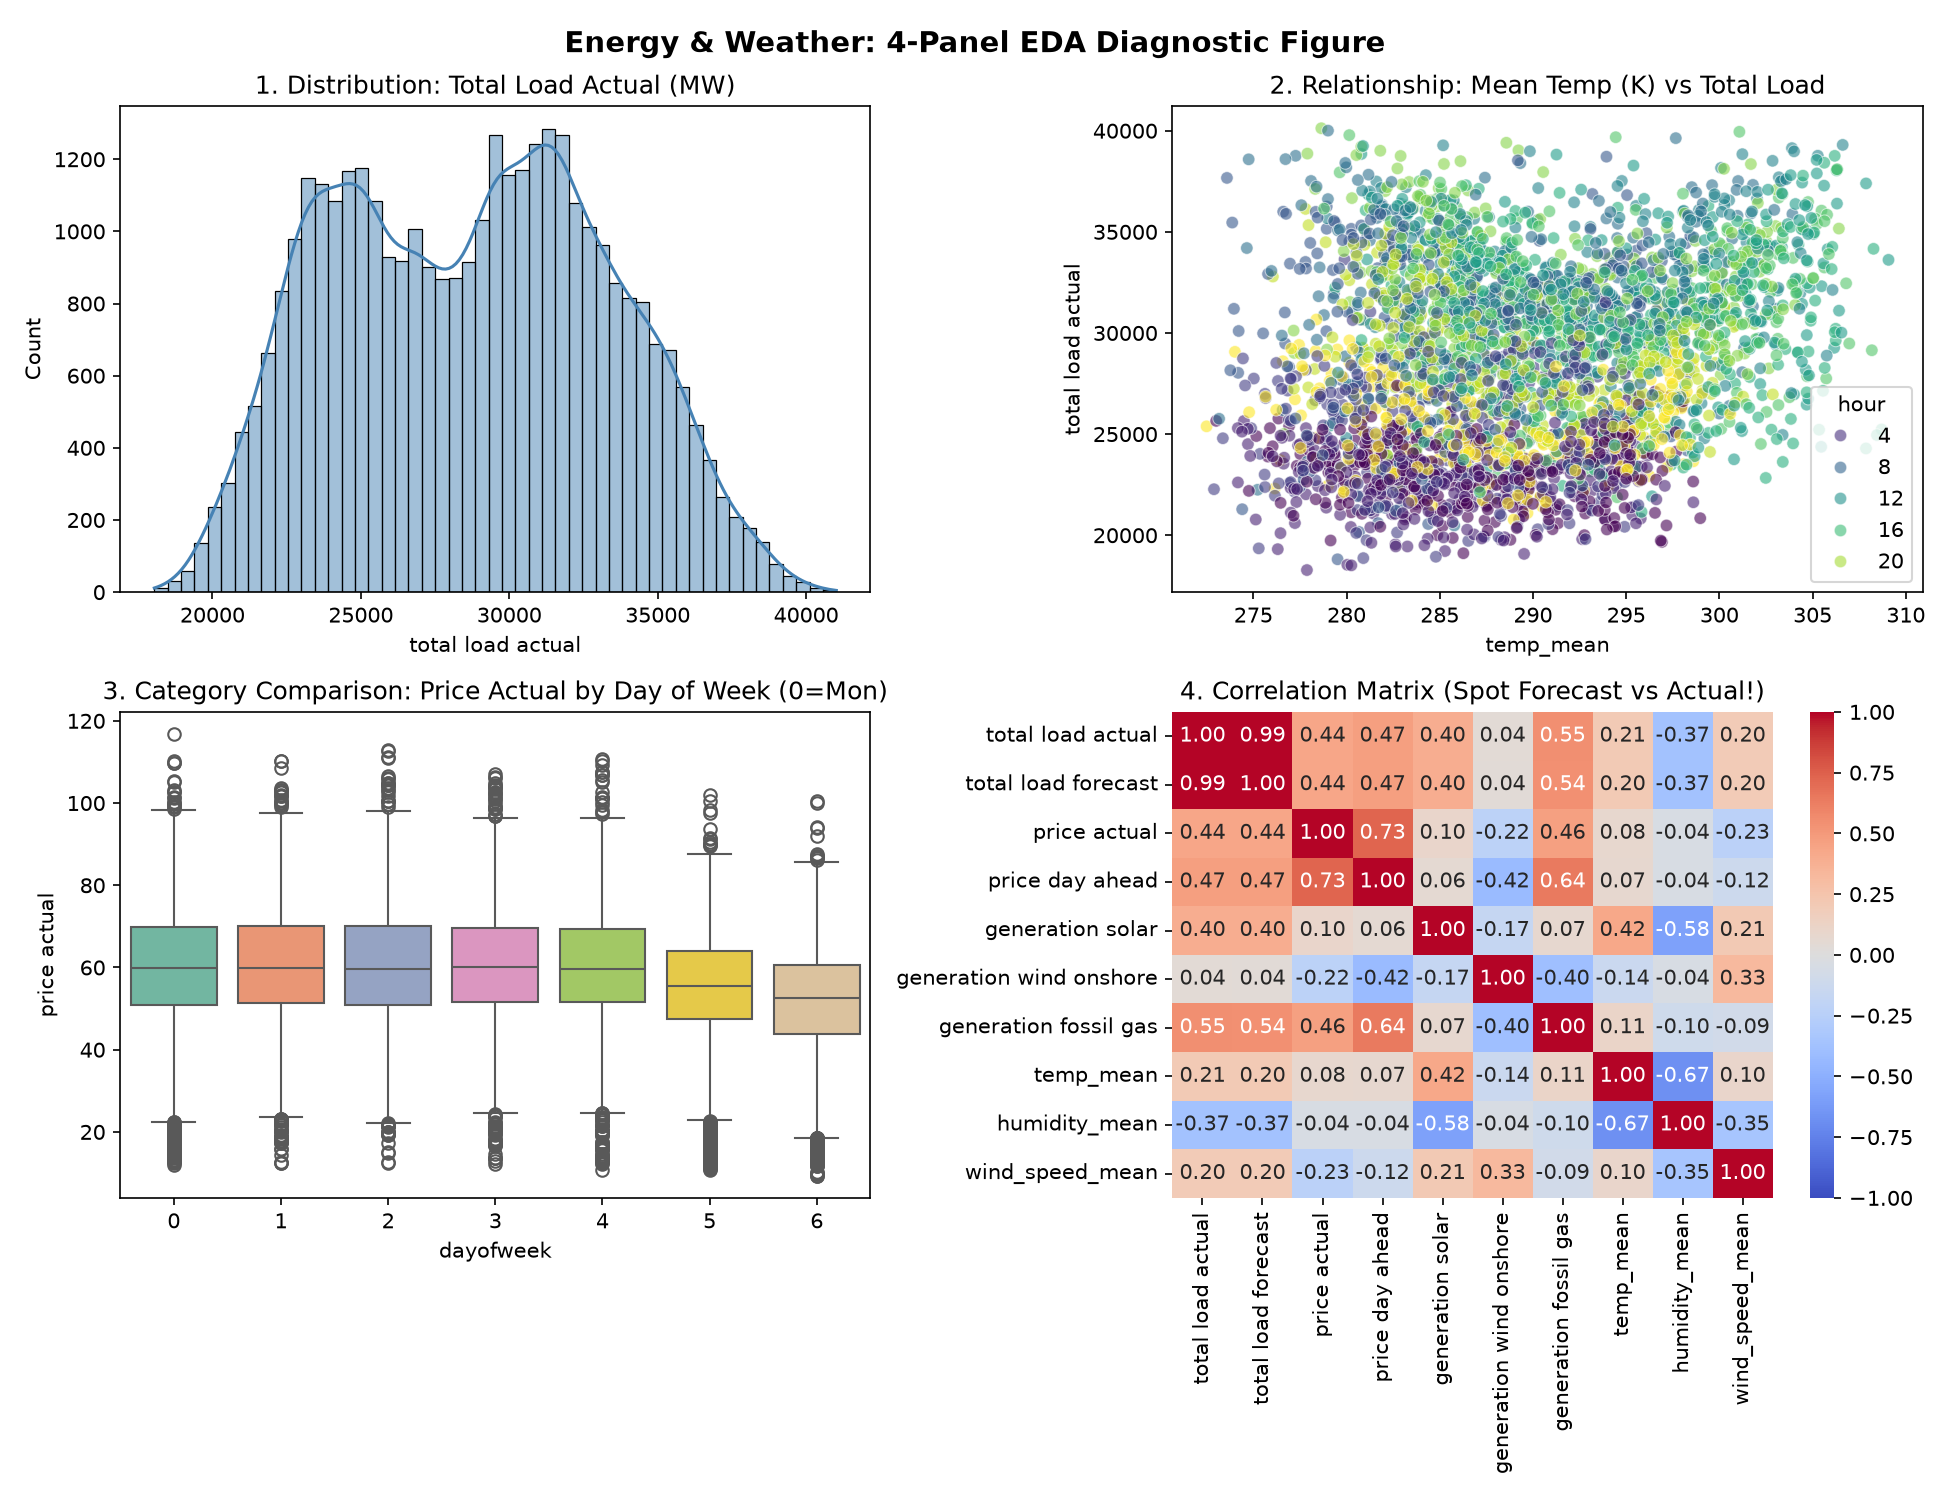
\includegraphics[width=0.92\linewidth]{eda_4panel.png}
\caption{Biểu đồ EDA 4 ô (phần A): phân phối phụ tải, quan hệ nhiệt độ--phụ tải, giá theo thứ, ma trận tương quan.}
\label{fig:eda}
\end{figure}

\todo{A viết chi tiết mục 3: mô tả cột, quy trình làm sạch, EDA, lý do chia theo thời gian.}

\section{Phương pháp và mô hình}\label{sec:methods}
% ============================================================================
% Mục 4.1 - Người viết: B
% ============================================================================
\subsection{Xây dựng đặc trưng (Phần B)}\label{sec:features}

Mục này mô tả mô-đun \code{src/features.py}: từ ba tập train/val/test do phần A tạo ra, sinh ra
\textbf{39 đặc trưng} thuộc ba nhóm --- \emph{lịch}, \emph{độ trễ (lag)} và \emph{thời tiết} --- dùng chung
cho mọi mô hình của nhóm (C, D). Mục tiêu thiết kế là: (i) mỗi đặc trưng đều phải \emph{quan sát được tại
thời điểm phát hành dự báo}; (ii) có cơ sở miền (domain) rõ ràng; (iii) tái lập được và có kiểm thử tự động.

\subsubsection{Thiết lập bài toán và nguyên tắc chống rò rỉ}\label{sec:setup}

\paragraph{Chân trời dự báo.} Phần B chọn \textbf{dự báo trước một ngày} ($h=24$ giờ) làm bài toán chính,
vì đây là thiết lập thực tế của thị trường điện ngày tới (OMIE) và của đơn vị vận hành lưới (REE). Chân trời
được tham số hóa qua \code{FeatureConfig(horizon=h)}; \cref{sec:horizon} so sánh thêm $h=1$.

\paragraph{Nguyên tắc chống rò rỉ (data leakage).} Mọi đặc trưng tại hàng $t$ được xây dựng sao cho:
\begin{enumerate}
  \item \textbf{Độ trễ $\geq h$}: chỉ dùng $y_{t-k}$ với $k\geq h$. Với $h=24$, các độ trễ 1--3 giờ bị
        loại bỏ tự động (\code{effective_lags}) dù có trong cấu hình.
  \item \textbf{Cửa sổ trượt kết thúc tại $t-h$}: thống kê trượt (trung bình, độ lệch chuẩn, min, max)
        được tính trên chuỗi đã dịch $y_{t-h}$, không bao giờ chứa $y_t$.
  \item \textbf{Tính trên trục thời gian liên tục}: ba tập được nối theo thứ tự thời gian, tính đặc trưng,
        rồi cắt lại theo mốc thời gian của phần A. Nhờ vậy 336 giờ đầu của tập validation vẫn có đặc trưng
        lag (lấy từ cuối tập train --- là quá khứ hợp lệ) và \textbf{không mất dòng nào} của val/test; chỉ
        672 giờ (4 tuần) đầu của tập train bị loại do chưa đủ lịch sử.
  \item \textbf{Loại các cột không có tại thời điểm dự báo}: các cột sản lượng phát (\code{generation *}),
        giá (\code{price actual}) phản ánh chính phụ tải giờ $t$; cột \code{total load forecast} là dự báo
        của TSO (tương quan 0.99 với mục tiêu, \cref{fig:eda}). Các cột này \emph{không bao giờ} là đầu vào;
        riêng \code{total load forecast} chỉ dùng làm mốc tham chiếu (\cref{sec:baselines}).
  \item \textbf{Chuẩn hóa nằm trong pipeline mô hình}: \code{StandardScaler} chỉ được \code{fit} trên tập
        huấn luyện của từng lần fit (\cref{sec:linear}), không chuẩn hóa trước trên toàn bộ dữ liệu.
\end{enumerate}

\paragraph{Giả định về thời tiết.} Đặc trưng thời tiết tại giờ $t$ sử dụng giá trị \emph{quan sát} tại $t$,
tương đương giả định có dự báo thời tiết hoàn hảo cho ngày mai. Đây là giả định phổ biến trong nghiên cứu
STLF~\cite{hong2016probabilistic}; trong vận hành thực tế, sai số dự báo nhiệt độ sẽ làm sai số phụ tải tăng nhẹ.

\subsubsection{Nhóm 1 -- Đặc trưng lịch (15 đặc trưng)}\label{sec:feat-cal}

Dữ liệu gốc lưu thời gian theo UTC, và phần A trích \code{hour}, \code{dayofweek} theo UTC. Tuy nhiên hành vi
tiêu dùng điện bám theo \textbf{giờ địa phương}: Tây Ban Nha dùng CET (UTC+1) vào mùa đông và CEST (UTC+2) vào
mùa hè. Nếu dùng giờ UTC, đỉnh phụ tải buổi sáng sẽ ``trượt'' một giờ giữa hai mùa. Phần B vì vậy chuyển
sang múi giờ \code{Europe/Madrid} trước khi trích đặc trưng (\cref{lst:calendar}).

\begin{table}[H]
\centering
\caption{Đặc trưng lịch (tiền tố \code{cal_}).}\label{tab:feat-cal}
\small
\begin{tabularx}{\linewidth}{lX}
\toprule
Đặc trưng & Ý nghĩa\\
\midrule
\code{hour}, \code{dayofweek}, \code{month}, \code{dayofyear} & Giờ (0--23), thứ (0 = Thứ Hai), tháng, ngày trong năm, theo giờ địa phương.\\
\code{is_weekend} & 1 nếu Thứ Bảy/Chủ Nhật.\\
\code{is_holiday} & 1 nếu là ngày lễ quốc gia Tây Ban Nha (1/1, 6/1, Thứ Sáu Tuần Thánh, 1/5, 15/8, 12/10, 1/11, 6/12, 8/12, 25/12).\\
\code{is_offday} & Cuối tuần \emph{hoặc} ngày lễ --- ngày nghỉ nói chung.\\
\code{is_bridge} & Ngày ``cầu'' (\emph{puente}): ngày làm việc kẹp giữa hai ngày nghỉ, nhiều người nghỉ phép.\\
\code{is_dst} & 1 khi áp dụng giờ mùa hè (CEST); tính từ độ lệch giờ địa phương -- UTC.\\
\code{hour_sin/cos}, \code{dow_sin/cos}, \code{doy_sin/cos} & Mã hóa tuần hoàn $\sin(2\pi x/P)$, $\cos(2\pi x/P)$ với chu kỳ $P = 24, 7, 365.25$.\\
\bottomrule
\end{tabularx}
\end{table}

\paragraph{Tại sao cần mã hóa tuần hoàn?} Biến giờ dạng số nguyên coi 23h và 0h cách nhau 23 đơn vị, trong
khi thực tế chúng liền kề. Ánh xạ lên đường tròn đơn vị,
\begin{equation}
  x \mapsto \bigl(\sin(2\pi x/P),\ \cos(2\pi x/P)\bigr),
\end{equation}
bảo toàn khoảng cách tuần hoàn. Mô hình tuyến tính hưởng lợi nhiều nhất; mô hình cây vẫn dùng được cả hai
dạng. Với mô hình tuyến tính, ngoài dạng tuần hoàn, \code{hour}, \code{dayofweek}, \code{month} còn được
mã hóa one-hot và thêm tương tác \code{hour}~$\times$~\code{is_offday} (\cref{sec:linear}).

\begin{lstlisting}[caption={Trích đặc trưng lịch theo giờ địa phương (rút gọn từ \code{features.py}).},label={lst:calendar}]
local = df["time"].dt.tz_convert("Europe/Madrid")
local_date = local.dt.tz_localize(None).dt.normalize()
hour, dow = local.dt.hour, local.dt.day_of_week
is_holiday = local_date.isin(SPAIN_HOLIDAYS)
out["cal_is_offday"] = ((dow >= 5) | is_holiday).astype(int)
utc_offset = local.dt.tz_localize(None) - df["time"].dt.tz_localize(None)
out["cal_is_dst"] = (utc_offset == pd.Timedelta(hours=2)).astype(int)  # CEST
out["cal_hour_sin"] = np.sin(2 * np.pi * hour / 24)
\end{lstlisting}

\subsubsection{Nhóm 2 -- Đặc trưng độ trễ và cửa sổ trượt (13 đặc trưng)}\label{sec:feat-lag}

Phụ tải điện có quán tính và tính mùa vụ theo ngày/tuần, nên giá trị quá khứ là đặc trưng mạnh nhất. Với
$h=24$, tập độ trễ hiệu lực là $\{24, 48, 72, 168, 336\}$ giờ:

\begin{table}[H]
\centering
\caption{Đặc trưng độ trễ (với $h=24$). Ký hiệu $\tilde{y}_t = y_{t-h}$ là giá trị gần nhất quan sát được.}\label{tab:feat-lag}
\small
\begin{tabularx}{\linewidth}{lX}
\toprule
Đặc trưng & Công thức / Ý nghĩa\\
\midrule
\code{lag_24}, \code{lag_48}, \code{lag_72} & $y_{t-24}, y_{t-48}, y_{t-72}$: cùng giờ 1, 2, 3 ngày trước.\\
\code{lag_168}, \code{lag_336} & $y_{t-168}, y_{t-336}$: cùng giờ, cùng thứ 1 và 2 tuần trước.\\
\code{roll_mean_24}, \code{roll_std_24} & Trung bình, độ lệch chuẩn của $\tilde{y}$ trong 24 giờ: mức nền và biên độ của ngày gần nhất.\\
\code{roll_mean_168}, \code{roll_std_168} & Như trên với cửa sổ 1 tuần: mức nền theo tuần.\\
\code{roll_min_24}, \code{roll_max_24} & Đáy đêm và đỉnh ngày của ngày gần nhất.\\
\code{lag_same_hour_4w_mean} & $\frac14\sum_{k=1}^{4} y_{t-168k}$: trung bình cùng giờ cùng thứ của 4 tuần trước.\\
\code{diff_24} & $y_{t-24} - y_{t-48}$: xu hướng tăng/giảm giữa hai ngày gần nhất.\\
\bottomrule
\end{tabularx}
\end{table}

\begin{lstlisting}[caption={Đặc trưng độ trễ luôn dịch ít nhất $h$ giờ.},label={lst:lags}]
y = df[TARGET]
for lag in cfg.effective_lags:            # only lags >= horizon
    out[f"lag_{lag}"] = y.shift(lag)
base = y.shift(cfg.horizon)                # last observable value
for w in cfg.roll_windows:                 # (24, 168)
    out[f"roll_mean_{w}"] = base.rolling(w, min_periods=w).mean()
    out[f"roll_std_{w}"]  = base.rolling(w, min_periods=w).std()
\end{lstlisting}

\subsubsection{Nhóm 3 -- Đặc trưng thời tiết (11 đặc trưng)}\label{sec:feat-weather}

EDA của phần A (\cref{fig:eda}, ô 2) cho thấy quan hệ nhiệt độ--phụ tải có dạng \textbf{chữ U}: phụ tải tăng
khi trời lạnh (sưởi) và khi trời nóng (điều hòa), thấp nhất quanh 15--19\,°C. Một hệ số tuyến tính duy nhất
cho nhiệt độ không thể biểu diễn quan hệ này, nên phần B xây dựng các biến đổi phi tuyến dựa trên khái niệm
\emph{độ-giờ sưởi/làm mát} (heating/cooling degree hours) quen thuộc trong ngành năng lượng:
\begin{align}
  \mathrm{HDH}_t &= \max\bigl(0,\ T_{\text{base}} - T_t\bigr), \qquad T_{\text{base}} = 18\,^\circ\mathrm{C},\\
  \mathrm{CDH}_t &= \max\bigl(0,\ T_t - (T_{\text{base}} + 4)\bigr),
\end{align}
trong đó $T_t$ là nhiệt độ trung bình 5 thành phố (đổi từ Kelvin sang °C). Khoảng 18--22\,°C là ``vùng thoải
mái'' không cần sưởi hay làm mát.

\begin{table}[H]
\centering
\caption{Đặc trưng thời tiết (tiền tố \code{w_}).}\label{tab:feat-weather}
\small
\begin{tabularx}{\linewidth}{lX}
\toprule
Đặc trưng & Ý nghĩa\\
\midrule
\code{temp_c} & Nhiệt độ trung bình (°C).\\
\code{temp_c_sq} & $(T_t - 18)^2$: thành phần bậc hai mô tả dạng chữ U.\\
\code{hdh}, \code{cdh} & Độ-giờ sưởi và làm mát (hàm hinge, tuyến tính từng khúc).\\
\code{temp_range} & $T_{\max} - T_{\min}$ giữa các thành phố: mức độ chênh lệch nhiệt vùng miền.\\
\code{humidity}, \code{pressure}, \code{wind_speed}, \code{clouds} & Độ ẩm, áp suất, gió, mây (trung bình 5 thành phố).\\
\code{temp_roll24} & Nhiệt độ trung bình 24 giờ qua: \emph{quán tính nhiệt} của tòa nhà.\\
\code{temp_roll24_diff} & $T_t - \overline{T}_{24h}$: thay đổi nhiệt đột ngột so với ngày trước.\\
\bottomrule
\end{tabularx}
\end{table}

\paragraph{Lưu ý về \code{temp_dev_mean} của phần A.} Cột này được tính bằng cách trừ nhiệt độ trung bình
của từng thành phố trên \emph{toàn bộ} 4 năm, tức có dùng thông tin của tập test. Phần B không dùng cột này để
tránh rò rỉ (dù mức độ rò rỉ nhỏ, chỉ là một hằng số theo thành phố).

\subsubsection{Kiểm thử tự động}\label{sec:feat-tests}

File \code{tests/test_features_and_evaluate.py} bổ sung các kiểm thử cho phần B:
\begin{itemize}
  \item \textbf{Không nhìn trước tương lai}: trên một chuỗi tổng hợp $y_t = t + c$, kiểm tra
        \code{lag_k}$\,= y_t - k$, cửa sổ trượt kết thúc đúng tại $t-h$ và không đặc trưng lag nào
        $\geq y_t$, với cả $h=1$ và $h=24$.
  \item \textbf{Múi giờ và ngày lễ}: 08:00 UTC ngày 1/1/2018 phải là 9h địa phương và là ngày lễ;
        22:30 UTC ngày 15/7/2018 phải là 0h ngày 16/7 (Thứ Hai) trong giờ mùa hè.
  \item \textbf{Trên dữ liệu thật}: val/test giữ đủ 5\,260 dòng, không còn NaN, các tập không chồng lấn.
  \item Mục tiêu, dự báo TSO và cột thời gian không lọt vào danh sách đặc trưng.
\end{itemize}

% Kết quả thực nghiệm của phần B (chạy bằng src/train_models.py)
\subsubsection{Đánh giá đóng góp của từng nhóm đặc trưng (ablation)}\label{sec:ablation}

Để kiểm chứng các nhóm đặc trưng có thực sự hữu ích, phần B huấn luyện Random Forest (100 cây, siêu tham số tốt
nhất ở \cref{sec:rf}) và Ridge ($\alpha=1$) trên tập train với từng tổ hợp nhóm đặc trưng, rồi đo trên tập
validation ($h=24$).

\begin{table}[H]
\centering
\caption{Ablation nhóm đặc trưng -- sai số trên tập validation ($h=24$). In đậm: tốt nhất mỗi cột.}\label{tab:ablation}
\small
\setlength{\tabcolsep}{5pt}
\begin{tabular}{lrrrrr}
\toprule
& & \multicolumn{2}{c}{Random Forest} & \multicolumn{2}{c}{Ridge}\\
\cmidrule(lr){3-4}\cmidrule(lr){5-6}
Nhóm đặc trưng & Số ĐT & MAE (MW) & MAPE (\%) & MAE (MW) & MAPE (\%)\\
\midrule
Chỉ thời tiết & 11 & 3\,370 & 11.63 & 3\,507 & 12.12\\
Chỉ lag & 13 & 1\,825 & 6.36 & 2\,012 & 7.03\\
Chỉ lịch & 15 & 1\,798 & 6.06 & 2\,064 & 7.04\\
Lag + thời tiết & 24 & 1\,875 & 6.51 & 2\,024 & 7.04\\
Lịch + thời tiết & 26 & 1\,736 & 5.91 & 2\,074 & 7.07\\
Lịch + lag & 28 & 1\,545 & 5.29 & \textbf{1\,852} & \textbf{6.39}\\
\textbf{Tất cả (3 nhóm)} & 39 & \textbf{1\,536} & \textbf{5.28} & 1\,870 & 6.44\\
\bottomrule
\end{tabular}
\end{table}

\paragraph{Nhận xét.}
\begin{itemize}
  \item \textbf{Lịch và lag bổ trợ cho nhau}: mỗi nhóm riêng lẻ cho MAE khoảng 1\,800~MW, nhưng kết hợp thì
        giảm còn 1\,545~MW ($-14\%$). Lag cho biết \emph{mức} phụ tải gần đây; lịch cho biết \emph{hình dạng}
        trong ngày và ngày nghỉ --- điều mà lag 24 giờ không biết (ví dụ dự báo cho Thứ Hai bằng dữ liệu Chủ Nhật).
  \item \textbf{Thời tiết đứng riêng rất yếu} (MAPE 11.6\%) vì không biết giờ trong ngày, nhưng thêm vào
        lịch thì vẫn giảm MAE từ 1\,798 xuống 1\,736~MW với Random Forest. Khi đã có lag, phần lớn thông tin
        thời tiết đã ``nằm sẵn'' trong phụ tải hôm qua (nhiệt độ thay đổi chậm), nên đóng góp biên chỉ còn
        $\approx 9$~MW.
  \item \textbf{Với Ridge, thêm thời tiết làm tệ đi nhẹ} (1\,852 $\to$ 1\,870~MW): quan hệ nhiệt độ--phụ tải
        phụ thuộc giờ trong ngày (\cref{fig:eda}, ô 2) mà mô hình tuyến tính cộng tính không biểu diễn được,
        nên các biến thời tiết chủ yếu thêm nhiễu. Đây là một lý do mô hình cây vượt trội ở \cref{sec:compare-c}.
\end{itemize}
Bộ đặc trưng đầy đủ 39 biến được giữ làm mặc định vì tốt nhất với mô hình phi tuyến (cũng là họ mô hình
boosting của phần D), còn Ridge tự co các hệ số thừa nhờ điều chuẩn.

\subsubsection{Độ quan trọng của đặc trưng}\label{sec:importance}

\Cref{fig:perm-imp} cho thấy \emph{permutation importance} của Random Forest: mức tăng MAE trên tập validation
khi xáo trộn ngẫu nhiên một cột (5 lần lặp). Khác với độ quan trọng theo độ giảm impurity --- vốn thiên vị các
biến liên tục/nhiều giá trị~\cite{strobl2007bias} --- permutation importance đo trực tiếp đóng góp vào sai số
trên dữ liệu chưa thấy.

\begin{figure}[H]
\centering
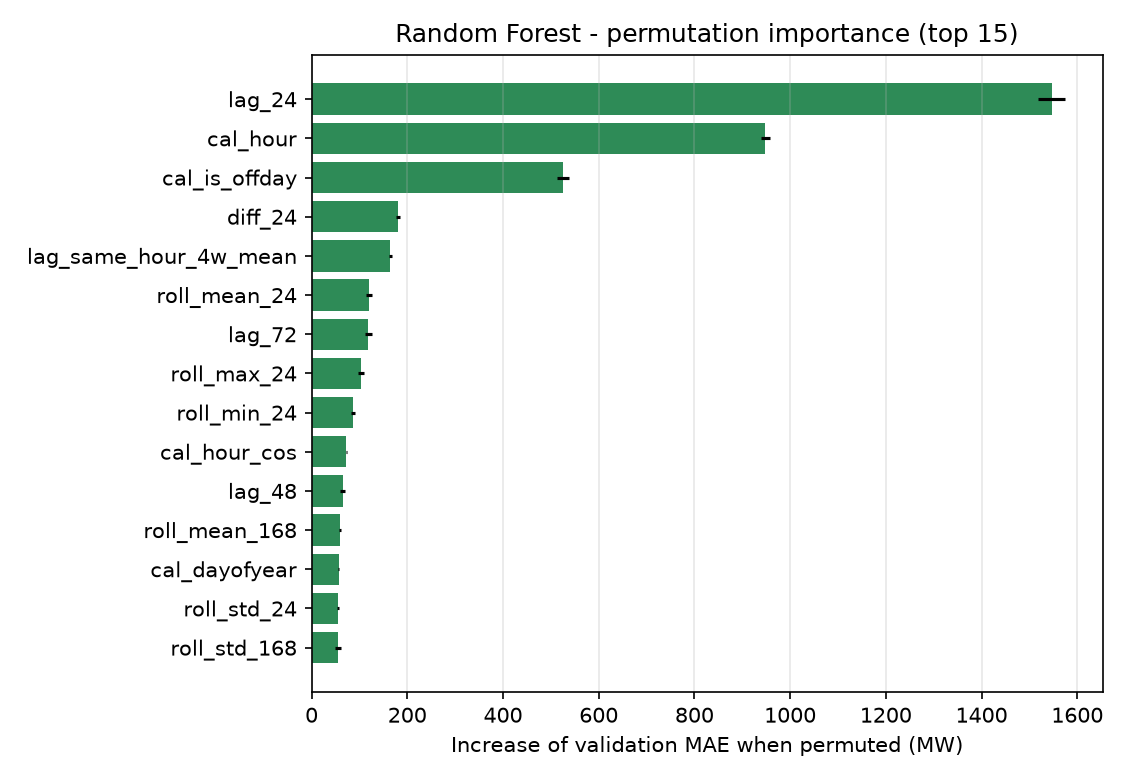
\includegraphics[width=0.8\linewidth]{b_feature_importance_rf.png}
\caption{Permutation importance (top 15) của Random Forest trên tập validation.}
\label{fig:perm-imp}
\end{figure}

Ba đặc trưng quan trọng nhất đến từ cả ba ý tưởng chính của phần B:
\code{lag_24} (+1\,546~MW khi bị xáo trộn), \code{cal_hour} (+948~MW) và \code{cal_is_offday} (+525~MW) ---
chính là biến ngày nghỉ tự xây dựng (cuối tuần \emph{hoặc} lễ). Tiếp theo là các đặc trưng lag phái sinh
(\code{diff_24}, \code{lag_same_hour_4w_mean}, \code{roll_mean_24}). Chỉ số impurity lại xếp \code{cal_hour}
cao nhất (0.45 so với 0.14 của \code{lag_24}), minh họa sự thiên vị nói trên.

\subsubsection{Ảnh hưởng của chân trời dự báo}\label{sec:horizon}

\begin{table}[H]
\centering
\caption{So sánh dự báo trước 1 giờ và trước 24 giờ (tập validation, cùng bộ đặc trưng và siêu tham số).}\label{tab:horizon}
\begin{tabular}{llrrr}
\toprule
Chân trời & Mô hình & MAE (MW) & RMSE (MW) & MAPE (\%)\\
\midrule
\multirow{3}{*}{$h=1$} & Ngây thơ $y_{t-1}$ & 1\,115 & 1\,507 & 3.91\\
 & Ridge & 405 & 677 & 1.42\\
 & Random Forest & \textbf{310} & \textbf{531} & \textbf{1.07}\\
\midrule
\multirow{3}{*}{$h=24$} & Ngây thơ $y_{t-24}$ & 2\,429 & 3\,507 & 8.43\\
 & Ridge & 1\,856 & 2\,513 & 6.39\\
 & Random Forest & \textbf{1\,536} & \textbf{2\,282} & \textbf{5.28}\\
\bottomrule
\end{tabular}
\end{table}

Khi được dùng $y_{t-1}$, mọi mô hình tốt hơn khoảng 5 lần. Điều này cho thấy hai điều: (i) chọn chân trời
là quyết định thiết kế quan trọng nhất và \textbf{phải được nêu rõ} khi so sánh với các kết quả khác --- nhiều
notebook công khai trên bộ dữ liệu này dùng lag 1 giờ nên có sai số thấp hơn nhiều; (ii) với $h=1$, Random
Forest đạt MAPE 1.07\%, xấp xỉ dự báo của TSO (1.05\%), gợi ý rằng dự báo TSO trong dữ liệu được cập nhật gần
thời gian thực chứ không phải dự báo ngày tới thuần túy (\cref{sec:baselines}).

\subsubsection{Một quan sát về chất lượng dữ liệu}\label{sec:data-quirk}

Khi phân tích sai số lớn nhất (\cref{sec:error-analysis}), phần B phát hiện chuỗi phụ tải có \textbf{tính mùa vụ
theo tuần yếu bất thường}: tự tương quan của phụ tải trung bình ngày ở độ trễ 7 ngày chỉ là 0.27 (nhỏ hơn
cả độ trễ 1 ngày, 0.37), và phụ tải trung bình Chủ Nhật chỉ thấp hơn Thứ Tư khoảng 12\%. Có những ngày cuối tuần
mang mức phụ tải của ngày làm việc (ví dụ Thứ Bảy 02/06/2018 trung bình 34\,328~MW, cao hơn mọi ngày trong
tuần trước đó) và ngược lại (Thứ Ba 05/06/2018 chỉ 23\,287~MW). Cột \code{total load forecast} của TSO cũng
bám đúng các bất thường này. Đây là đặc tính của dữ liệu nguồn chứ không phải lỗi của pipeline (các mốc thời
gian và tính liên tục theo giờ đã được kiểm tra), nhưng nó giới hạn độ chính xác mà các đặc trưng lịch có thể
mang lại. Nhóm đề xuất phần A kiểm tra thêm với dữ liệu gốc từ ENTSO-E/REE.


% ============================================================================
% Mục 4.2 - Người viết: C
% ============================================================================
\subsection{Mô hình cơ sở, Ridge/Lasso và Random Forest (Phần C)}\label{sec:models-c}

Phần C xây dựng: (i) mô-đun đánh giá dùng chung \code{src/evaluate.py} để \emph{mọi} mô hình của nhóm được
chấm điểm cùng một cách; (ii) các mô hình cơ sở (baseline); (iii) hồi quy tuyến tính có điều chuẩn Ridge và
Lasso; (iv) Random Forest. Mã nguồn huấn luyện nằm ở \code{src/train_models.py}; toàn bộ thí nghiệm chạy trong
khoảng 13 phút trên CPU 12 luồng.

\subsubsection{Mô-đun đánh giá dùng chung \code{evaluate.py}}\label{sec:evaluate}

Với $n$ giờ, giá trị thực $y_i$ và dự báo $\hat{y}_i$, mô-đun tính sáu chỉ số:
\begin{align}
\mathrm{MAE} &= \frac1n\sum_{i=1}^n |y_i-\hat y_i|, &
\mathrm{RMSE} &= \sqrt{\frac1n\sum_{i=1}^n (y_i-\hat y_i)^2},\\
\mathrm{MAPE} &= \frac{100}{n}\sum_{i=1}^n \left|\frac{y_i-\hat y_i}{y_i}\right|, &
\mathrm{sMAPE} &= \frac{100}{n}\sum_{i=1}^n \frac{|y_i-\hat y_i|}{(|y_i|+|\hat y_i|)/2},\\
R^2 &= 1-\frac{\sum_i (y_i-\hat y_i)^2}{\sum_i (y_i-\bar y)^2}, &
\mathrm{MaxAE} &= \max_i |y_i-\hat y_i|.
\end{align}

\paragraph{Lý do chọn chỉ số.} \textbf{MAE} (đơn vị MW) dễ diễn giải với người vận hành và là tiêu chí
chọn siêu tham số; \textbf{RMSE} phạt nặng các giờ sai lớn --- vốn gây tốn kém nhất (huy động dự phòng);
\textbf{MAPE} không phụ thuộc thang đo, dùng được vì phụ tải luôn $\geq 18\,000$~MW nên không có vấn đề chia
cho số gần 0~\cite{hyndman2006accuracy}; \textbf{MaxAE} cho biết giờ tệ nhất.

\paragraph{Thiết kế.} Mô-đun gồm:
\begin{itemize}
  \item Các hàm chỉ số thuần NumPy, kiểm tra đầu vào (khác kích thước, NaN/inf, MAPE khi $y=0$ đều báo lỗi
        thay vì âm thầm trả về số sai).
  \item Lớp \code{ResultsLog} tích lũy các dòng (mô hình, tập, chỉ số) và xuất bảng/CSV --- phần D và E chỉ
        cần gọi \code{log.add(...)} là có kết quả cùng định dạng với \cref{tab:main-results}.
  \item Các hàm chẩn đoán: \code{error_by_group} (MAE theo giờ/thứ/tháng địa phương), \code{plot_forecast},
        \code{plot_residuals}, \code{plot_metric_bars}.
\end{itemize}

\begin{lstlisting}[caption={Cách dùng \code{evaluate.py} cho bất kỳ mô hình nào.},label={lst:evaluate}]
from evaluate import ResultsLog
log = ResultsLog()
log.add("Random Forest", "test", test[TARGET], rf.predict(test[cols]), family="tree")
log.to_frame()            # DataFrame: model, split, MAE, RMSE, MAPE, sMAPE, R2, MaxAE
log.save(Path("results/metrics.csv"))
\end{lstlisting}

\subsubsection{Giao thức thực nghiệm}\label{sec:protocol}

Mọi mô hình tuân theo cùng một giao thức, nhằm tránh chọn siêu tham số dựa trên tập test:
\begin{enumerate}
  \item \textbf{Tinh chỉnh}: fit trên \emph{train} (23\,872 giờ sau khi bỏ 4 tuần khởi động lag), chọn cấu hình
        có MAE nhỏ nhất trên \emph{validation} (5\,260 giờ).
  \item \textbf{Đánh giá cuối}: fit lại cấu hình đã chọn trên \emph{train + validation}, chấm điểm \emph{một lần}
        trên \emph{test} (5\,260 giờ, 26/05--31/12/2018).
\end{enumerate}
Không dùng k-fold ngẫu nhiên vì sẽ trộn tương lai vào tập huấn luyện~\cite{bergmeir2012cv}. Fit lại trên
train+val giúp mô hình thấy dữ liệu gần tập test nhất (mùa đông 2017--2018), điều quan trọng với chuỗi có xu hướng.

\subsubsection{Các mô hình cơ sở}\label{sec:baselines}

Mô hình cơ sở cho biết một mô hình học máy có thực sự ``học'' được gì hay không~\cite{hyndman2021fpp3}:
\begin{itemize}
  \item \textbf{Ngây thơ theo ngày}: $\hat y_t = y_{t-24}$ (cùng giờ hôm qua).
  \item \textbf{Ngây thơ theo mùa (tuần)}: $\hat y_t = y_{t-168}$ (cùng giờ, cùng thứ tuần trước) --- xử lý
        được chuyển tiếp cuối tuần/đầu tuần.
  \item \textbf{Trung bình 4 tuần}: $\hat y_t = \frac14\sum_{k=1}^4 y_{t-168k}$ --- giảm nhiễu của một tuần đơn lẻ.
  \item \textbf{Dự báo của TSO} (\code{total load forecast}, \emph{chỉ để tham chiếu}): đây là dự báo do đơn vị
        vận hành lưới công bố, có dùng thông tin mà nhóm không có. Như phân tích ở \cref{sec:horizon}, sai số
        của nó tương đương mô hình dự báo trước 1 giờ, nên \textbf{không phải đối thủ công bằng} cho bài toán
        $h=24$; nó cho biết giới hạn trên thực tế.
\end{itemize}
Các baseline không cần huấn luyện nên chúng được tính trực tiếp từ các cột lag của \cref{sec:feat-lag}.

\subsubsection{Ridge và Lasso}\label{sec:linear}

Hồi quy tuyến tính với điều chuẩn $\ell_2$ (Ridge~\cite{hoerl1970ridge}) và $\ell_1$ (Lasso~\cite{tibshirani1996lasso}):
\begin{align}
\hat\beta^{\text{Ridge}} &= \arg\min_\beta\ \|y - X\beta\|_2^2 + \alpha\|\beta\|_2^2,\\
\hat\beta^{\text{Lasso}} &= \arg\min_\beta\ \tfrac{1}{2n}\|y - X\beta\|_2^2 + \alpha\|\beta\|_1.
\end{align}
Các đặc trưng lag tương quan rất mạnh với nhau (\code{lag_24}, \code{roll_mean_24}, \code{roll_max_24},\dots),
nên OLS thuần sẽ có hệ số không ổn định; Ridge co các hệ số về 0 để ổn định, còn Lasso có thể đưa hẳn hệ số về
0, tức tự chọn đặc trưng.

\paragraph{Tiền xử lý trong pipeline.} Mô hình tuyến tính không tự học được tương tác, nên phần C dùng
\code{ColumnTransformer} gồm: \code{StandardScaler} cho 35 biến số và \code{OneHotEncoder} (bỏ mức đầu) cho
4 biến phân loại: \code{cal_hour}, \code{cal_dayofweek}, \code{cal_month} và tương tác
\code{cal_hour}~$\times$~\code{cal_is_offday} (48 mức) --- cho phép hình dạng phụ tải trong ngày khác nhau giữa
ngày làm việc và ngày nghỉ. Tổng cộng 123 hệ số. Vì scaler nằm trong \code{Pipeline}, nó chỉ học trung bình/độ
lệch chuẩn từ dữ liệu được \code{fit}.

\paragraph{Tinh chỉnh $\alpha$.} Ridge: 13 giá trị $\alpha\in[10^{-2},10^{4}]$ (thang log); Lasso: 8 giá trị
$\alpha\in[10^{-1},10^{2.5}]$. Kết quả ở \cref{fig:tuning-linear}: chọn $\alpha^{\text{Ridge}}=100$ (MAE val
1\,856~MW) và $\alpha^{\text{Lasso}}=3.16$ (1\,850~MW). Đường cong khá phẳng với $\alpha$ nhỏ, cho thấy
điều chuẩn chỉ cải thiện nhẹ (~15~MW); $\alpha$ quá lớn làm mô hình underfit rõ rệt. Lasso giữ lại
\textbf{82/123} hệ số khác 0; các hệ số lớn nhất là các mức giờ tối (20--22h), \code{lag_24}, các tương tác
giờ~$\times$~ngày nghỉ và tháng 7 (điều hòa mùa hè) --- phù hợp trực giác.

\begin{figure}[H]
\centering
\begin{subfigure}{0.49\linewidth}
  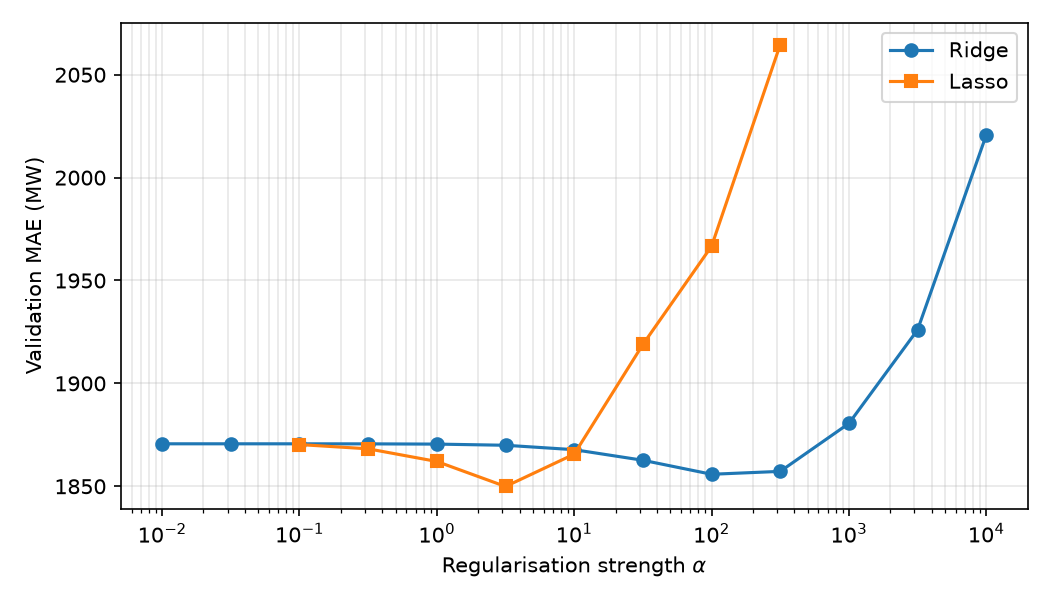
\includegraphics[width=\linewidth]{c_tuning_linear.png}
  \caption{Ridge / Lasso theo $\alpha$.}\label{fig:tuning-linear}
\end{subfigure}\hfill
\begin{subfigure}{0.49\linewidth}
  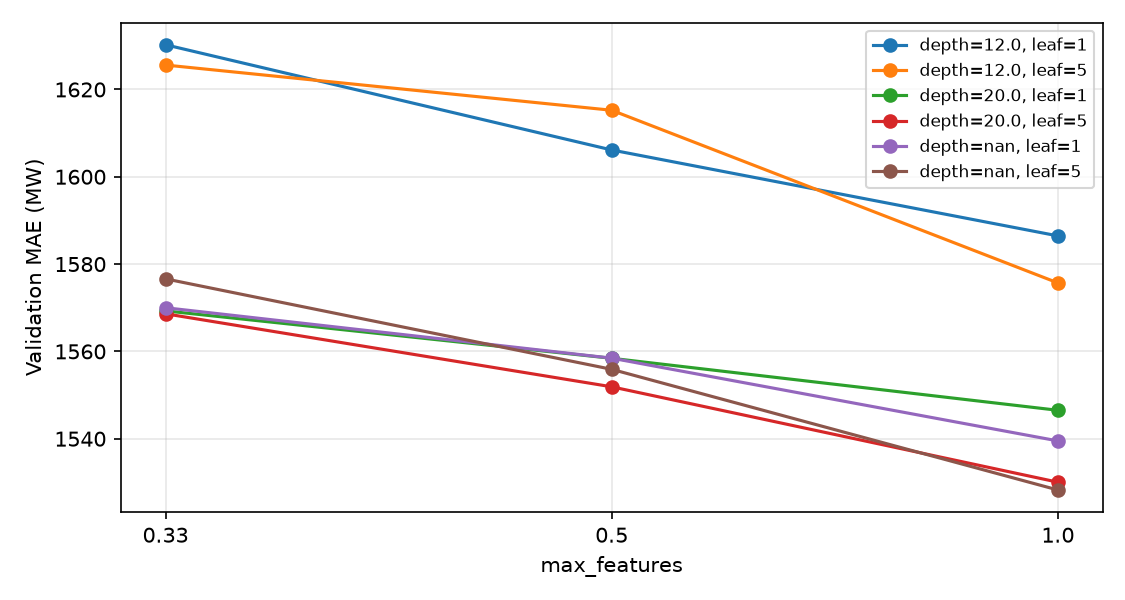
\includegraphics[width=\linewidth]{c_tuning_rf.png}
  \caption{Random Forest theo lưới siêu tham số.}\label{fig:tuning-rf}
\end{subfigure}
\caption{Đường cong tinh chỉnh trên tập validation (MAE).}
\end{figure}

\subsubsection{Random Forest}\label{sec:rf}

Random Forest~\cite{breiman2001random} là trung bình của $B$ cây hồi quy, mỗi cây học trên một mẫu bootstrap và
tại mỗi nút chỉ xét ngẫu nhiên \code{max_features} đặc trưng:
\begin{equation}
\hat y(x) = \frac1B\sum_{b=1}^B T_b(x).
\end{equation}
Mô hình tự học tương tác (giờ~$\times$~ngày nghỉ~$\times$~nhiệt độ) và quan hệ phi tuyến chữ U mà không cần
thiết kế thủ công, không cần chuẩn hóa, và việc lấy trung bình giảm phương sai của từng cây.

\paragraph{Tinh chỉnh.} Lưới 18 cấu hình (200 cây mỗi cấu hình):
\code{max_depth}~$\in\{12, 20, \text{None}\}$, \code{min_samples_leaf}~$\in\{1,5\}$,
\code{max_features}~$\in\{0.33, 0.5, 1.0\}$. Cấu hình tốt nhất: \code{max_depth=None},
\code{min_samples_leaf=5}, \code{max_features=1.0} (MAE val 1\,528~MW). \Cref{fig:tuning-rf} cho thấy: cây sâu
hơn luôn tốt hơn (độ sâu 12 bị underfit), \code{min_samples_leaf=5} làm mượt lá và tốt hơn 1 một chút, và
\code{max_features=1.0} (tức bagging thuần) tốt nhất --- vì có ít đặc trưng thực sự mạnh (\code{lag_24},
\code{cal_hour}), buộc cây bỏ qua chúng ở một nút làm giảm chất lượng nhiều hơn lợi ích giải tương quan.
Mô hình cuối dùng 500 cây.

\subsubsection{Kết quả}\label{sec:compare-c}

\begin{table}[H]
\centering
\caption{Kết quả dự báo trước 24 giờ. Validation: mô hình fit trên train. Test: fit trên train+val.
In đậm: tốt nhất trong các mô hình của nhóm.}\label{tab:main-results}
\small
\begin{tabular}{lrrrrrrrr}
\toprule
& \multicolumn{4}{c}{Validation} & \multicolumn{4}{c}{Test}\\
\cmidrule(lr){2-5}\cmidrule(lr){6-9}
Mô hình & MAE & RMSE & MAPE & $R^2$ & MAE & RMSE & MAPE & $R^2$\\
\midrule
Ngây thơ $y_{t-24}$ & 2\,429 & 3\,507 & 8.43 & 0.445 & 2\,533 & 3\,622 & 8.76 & 0.378\\
Ngây thơ $y_{t-168}$ & 2\,571 & 3\,663 & 8.87 & 0.394 & 2\,589 & 3\,818 & 8.96 & 0.308\\
Trung bình 4 tuần & 2\,245 & 3\,019 & 7.85 & 0.589 & 2\,223 & 3\,029 & 7.68 & 0.565\\
Ridge ($\alpha=100$) & 1\,856 & 2\,513 & 6.39 & 0.715 & 1\,788 & 2\,520 & 6.14 & 0.699\\
Lasso ($\alpha=3.16$) & 1\,850 & 2\,507 & 6.37 & 0.716 & 1\,787 & 2\,524 & 6.14 & 0.698\\
\textbf{Random Forest} & \textbf{1\,527} & \textbf{2\,269} & \textbf{5.24} & \textbf{0.768} & \textbf{1\,530} & \textbf{2\,355} & \textbf{5.22} & \textbf{0.737}\\
\midrule
\textit{Dự báo TSO (tham chiếu)} & \textit{304} & \textit{451} & \textit{1.05} & \textit{0.991} & \textit{255} & \textit{342} & \textit{0.87} & \textit{0.994}\\
\bottomrule
\end{tabular}
\\[2pt]\footnotesize MAE, RMSE tính bằng MW; MAPE tính bằng \%. File đầy đủ (gồm sMAPE, MaxAE): \code{results/metrics.csv}.
\end{table}

\begin{figure}[H]
\centering
\begin{subfigure}{0.49\linewidth}
  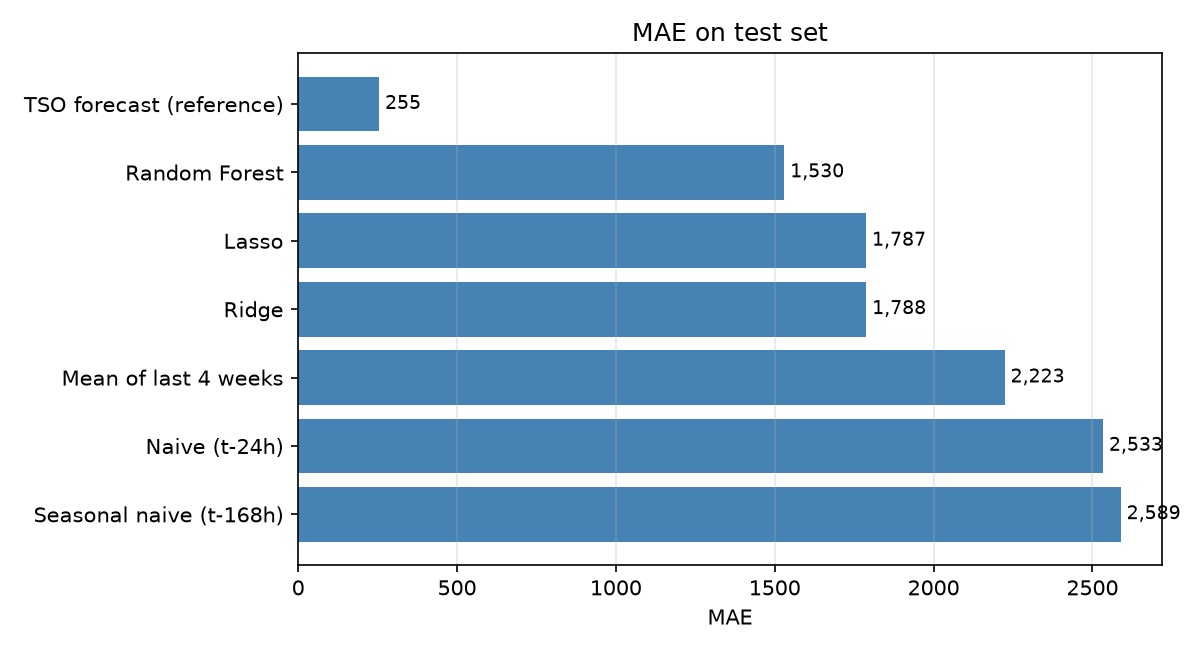
\includegraphics[width=\linewidth]{c_mae_test.png}
  \caption{MAE trên tập test.}
\end{subfigure}\hfill
\begin{subfigure}{0.49\linewidth}
  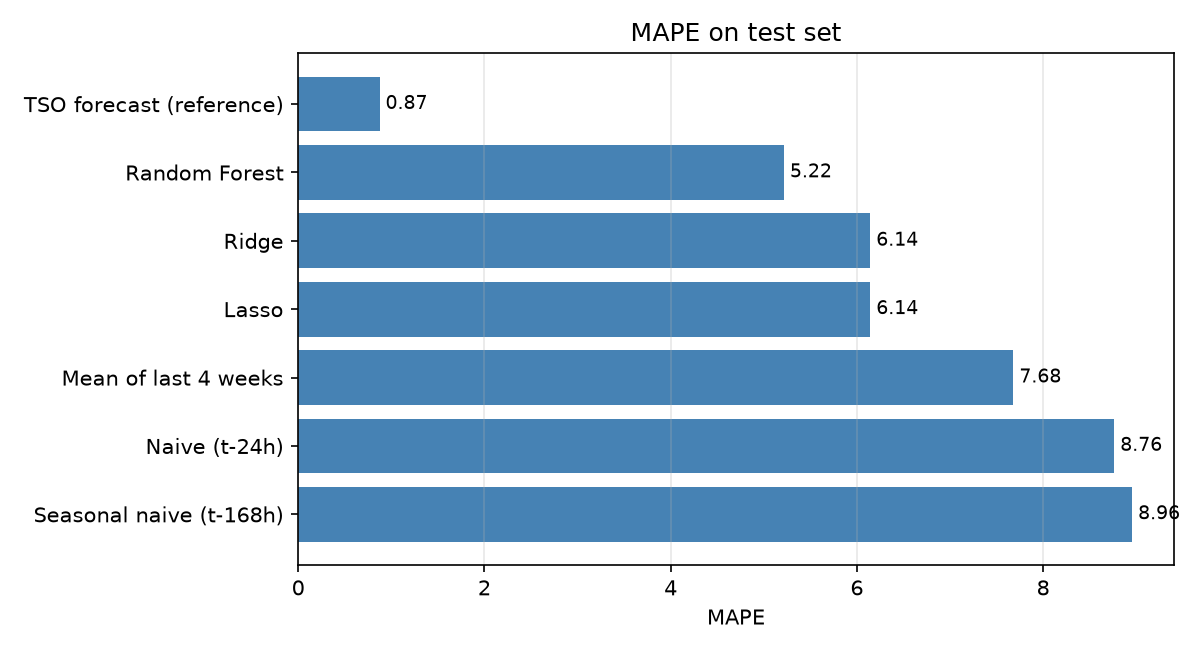
\includegraphics[width=\linewidth]{c_mape_test.png}
  \caption{MAPE trên tập test.}
\end{subfigure}
\caption{So sánh các mô hình của phần C trên tập test.}\label{fig:bars}
\end{figure}

\paragraph{Nhận xét chính.}
\begin{enumerate}
  \item \textbf{Mọi mô hình học máy đều vượt baseline.} Random Forest giảm MAE 39.6\% so với $y_{t-24}$ và
        31.2\% so với baseline tốt nhất (trung bình 4 tuần). Ridge/Lasso giảm 19.6\% so với baseline tốt nhất.
  \item \textbf{Random Forest tốt hơn tuyến tính 14.4\% MAE} nhờ học được tương tác và quan hệ phi tuyến.
        Khoảng cách RMSE nhỏ hơn (6.6\%), nghĩa là RF chủ yếu tốt hơn ở các giờ ``bình thường''; cả hai đều
        sai lớn ở các ngày bất thường.
  \item \textbf{Ridge và Lasso gần như như nhau} (chênh lệch $<1$~MW trên test): với 23\,872 mẫu và 123 hệ số,
        điều chuẩn chỉ đóng vai trò nhỏ; ưu điểm của Lasso là mô hình thưa hơn (82 hệ số).
  \item \textbf{Tổng quát hóa ổn định}: sai số val và test gần nhau (RF: 1\,527 vs 1\,530~MW), cho thấy giao
        thức tinh chỉnh không overfit tập validation. $R^2$ test thấp hơn val chủ yếu do phương sai của tập
        test nhỏ hơn (mùa hè--thu), không phải do sai số tăng.
  \item \textbf{Ngây thơ tuần kém hơn ngây thơ ngày}, trái với dữ liệu phụ tải thông thường --- một hệ quả của
        tính mùa vụ tuần yếu đã nêu ở \cref{sec:data-quirk}.
\end{enumerate}

\subsubsection{Phân tích sai số}\label{sec:error-analysis}

\begin{figure}[H]
\centering
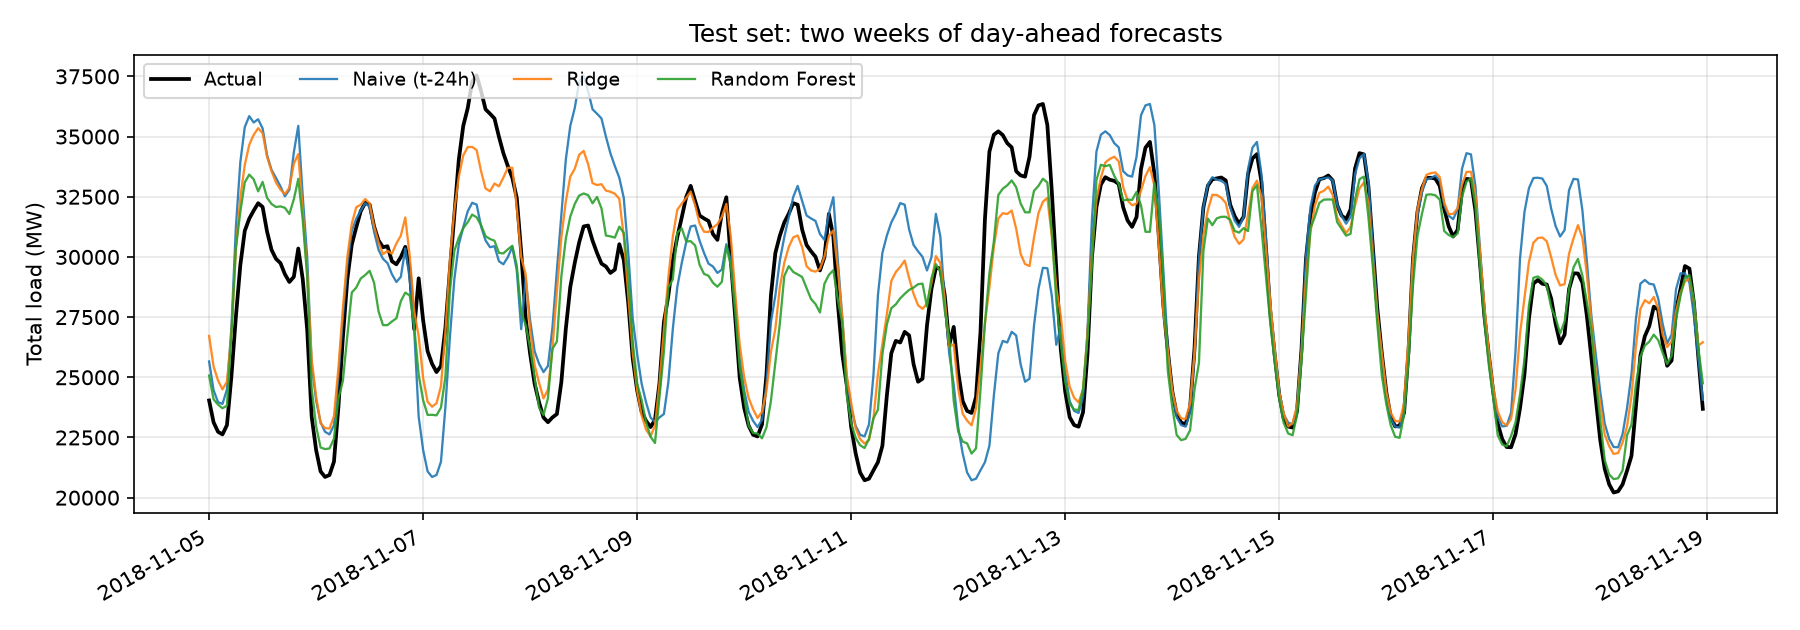
\includegraphics[width=\linewidth]{c_forecast_2weeks.png}
\caption{Hai tuần dự báo trên tập test, từ ngày 5 đến ngày 19 tháng 11 năm 2018.}\label{fig:forecast}
\end{figure}

\Cref{fig:forecast} cho thấy cả ba mô hình bám tốt hình dạng ngày (đáy đêm, đỉnh sáng và tối). Mô hình ngây
thơ ``trễ một ngày'' rõ rệt: khi một ngày có phụ tải bất thường (12/11), nó lặp lại bất thường đó vào ngày hôm
sau. Ridge và đặc biệt Random Forest giảm đáng kể lỗi lặp này nhờ kết hợp lag với lịch và trung bình nhiều tuần,
nhưng không thể đoán trước một ngày bất thường như 07/11 hay 12/11.

\begin{figure}[H]
\centering
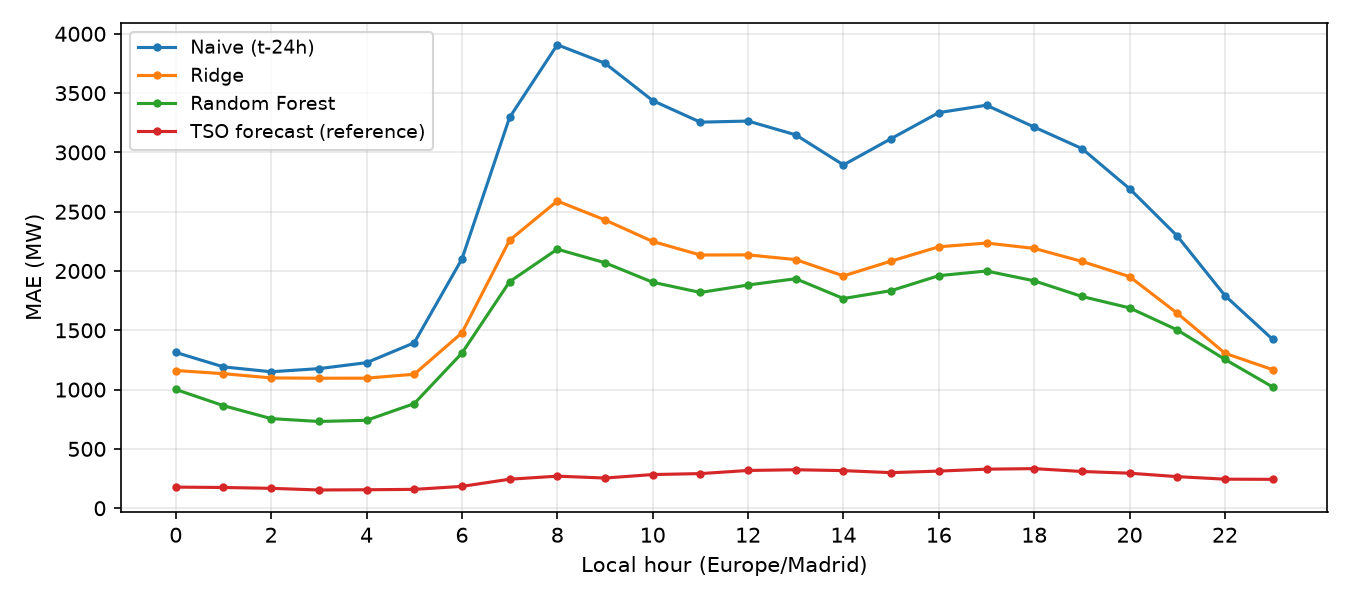
\includegraphics[width=0.85\linewidth]{c_mae_by_hour.png}
\caption{MAE theo giờ địa phương trên tập test.}\label{fig:mae-hour}
\end{figure}

\paragraph{Theo giờ (\cref{fig:mae-hour}).} Sai số nhỏ nhất vào 2--5h sáng (phụ tải nền ổn định, RF
$\approx 750$~MW) và lớn nhất vào 8h sáng (RF $\approx 2\,200$~MW) --- giờ tăng tải buổi sáng, nhạy với
việc ngày đó là ngày làm việc hay nghỉ. RF tốt hơn Ridge ở mọi giờ, rõ nhất vào ban đêm.

\paragraph{Theo thứ.} MAE test của RF thấp nhất vào Thứ Tư (1\,274~MW) và Thứ Sáu (1\,314~MW), cao nhất vào
Thứ Bảy (1\,723~MW) và Chủ Nhật (1\,988~MW). Baseline $y_{t-24}$ đặc biệt tệ vào Thứ Hai (4\,396~MW) vì dùng
phụ tải Chủ Nhật; RF giảm lỗi Thứ Hai xuống 1\,469~MW ($-67\%$) nhờ biến \code{cal_is_offday} và lag tuần.

\paragraph{Các giờ sai lớn nhất} tập trung vào một số ngày cuối tuần có phụ tải ở mức ngày làm việc (02/06,
01/09, 01/12/2018: sai tới 10\,000~MW) và Giáng Sinh 25/12 (dự báo cao hơn thực tế $\approx 9\,600$~MW lúc 8h).
Ngày lễ chỉ xuất hiện 2--3 lần mỗi năm trong train nên mô hình học được hiệu ứng ngày lễ chưa đủ mạnh.

\begin{figure}[H]
\centering
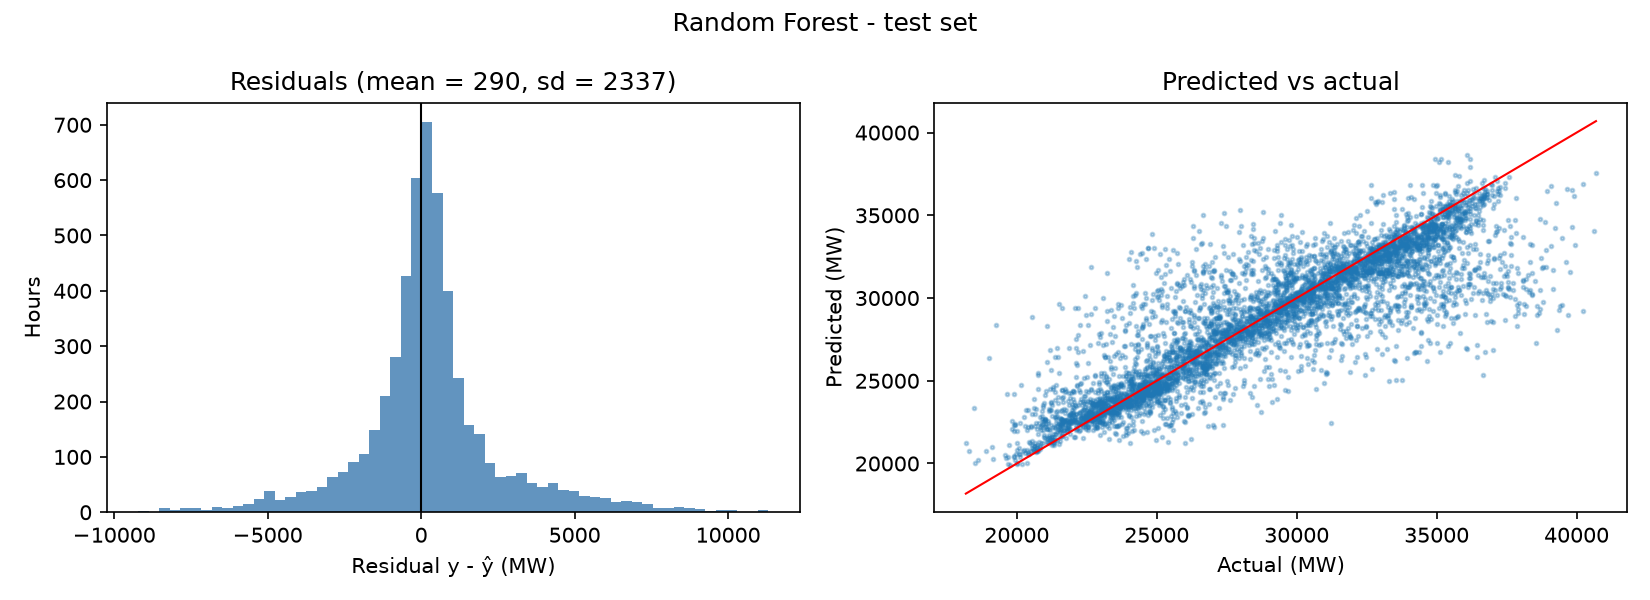
\includegraphics[width=0.95\linewidth]{c_residuals_rf.png}
\caption{Phần dư của Random Forest trên tập test.}\label{fig:residuals}
\end{figure}

\Cref{fig:residuals} cho thấy phần dư tập trung quanh 0 nhưng có đuôi dày ở cả hai phía --- tương ứng với các
ngày bất thường nói trên --- và mô hình có xu hướng ``co về trung bình'' ở các giờ phụ tải rất cao
(điểm nằm dưới đường chéo ở góc phải), một đặc điểm đã biết của Random Forest: dự báo là trung bình các lá nên
không ngoại suy vượt khoảng giá trị đã thấy.

\subsubsection{Hạn chế và đề xuất cho phần D, E}
\begin{itemize}
  \item Random Forest là mô hình tốt nhất của phần C và là \textbf{mốc để phần D (LightGBM/XGBoost) so sánh};
        boosting có thể giảm thêm thiên lệch ở các giờ cao tải.
  \item Dự báo TSO vẫn tốt hơn nhiều; một phần do TSO có thông tin cập nhật trong ngày. Với $h=1$, RF đạt MAPE
        1.07\% (\cref{tab:horizon}), ngang TSO.
  \item Cải tiến khả thi: đặc trưng ngày lễ vùng (Catalonia, Madrid, \dots), ``ngày sau lễ'', trọng số theo dân số
        cho thời tiết 5 thành phố, và dự báo xác suất (khoảng tin cậy) thay vì điểm.
\end{itemize}

\subsection{LightGBM, XGBoost và tinh chỉnh siêu tham số}\label{sec:boosting}
% Người viết: D
\todo{D viết mục 4.3. Dùng chung \code{features.make_datasets()} và \code{evaluate.ResultsLog} để kết quả
so sánh được với \cref{tab:main-results}; tuân theo cùng giao thức train$\to$val để tinh chỉnh, train+val$\to$test.}

% ============================================================================
% Mục 4.4 - Hiện thực mã nguồn của phần B (features.py) và C (evaluate.py)
% ============================================================================
\subsection{Hiện thực mã nguồn (Phần B và C)}\label{sec:impl}

Mục này mô tả chi tiết hai mô-đun dùng chung do phần B và C viết: \code{src/features.py} (đặc trưng) và
\code{src/evaluate.py} (đánh giá). Với mỗi file, báo cáo liệt kê các thư viện được import, các biến toàn cục
(global), các lớp và hàm, kèm giải thích đầu vào, đầu ra và cách hoạt động. Mô-đun huấn luyện
\code{train_models.py} chỉ \emph{gọi} hai mô-đun này nên không được mô tả lại ở đây.

\subsubsection{Tổng quan luồng gọi hàm}\label{sec:impl-flow}

\begin{lstlisting}[language={},numbers=none,caption={Luồng gọi hàm từ dữ liệu đã chia đến bảng kết quả.},label={lst:callgraph}]
features.make_datasets(cfg)
 |-- load_splits()                    -> {train, val, test} (Parquet from part A)
 |-- build_feature_frame(full, cfg)   -> time + target + TSO + 39 features
 |    |-- add_calendar_features(full)       15 columns cal_*
 |    |-- add_lag_features(full, cfg)       13 columns lag_*, roll_*, diff_24
 |    `-- add_weather_features(full, cfg)   11 columns w_*
 |-- cut back by train/val/test time bounds, dropna (lag warm-up)
 `-- feature_columns(frame)           -> list of model inputs

train_models.py: fit model on feature_columns -> y_pred
evaluate.ResultsLog.add(model, split, y_true, y_pred)
 `-- evaluate() -> mae, rmse, mape, smape, r2, max_ae  (each calls _as_arrays)
evaluate.plot_* / error_by_group  -> figures in plots/
\end{lstlisting}

\subsubsection{Các thư viện được import}\label{sec:impl-imports}

Hai mô-đun \textbf{không thêm thư viện bên thứ ba nào mới}: mọi gói đều đã có trong \code{pyproject.toml}
của phần A, nên \code{uv sync} không cần thay đổi. Các import ``mới'' (chưa xuất hiện trong
\code{data_preprocessing.py}) là \code{from __future__ import annotations} và \code{dataclasses.field}.

\begingroup\footnotesize
\begin{longtable}{>{\raggedright\arraybackslash}p{0.30\linewidth}>{\raggedright\arraybackslash}p{0.13\linewidth}>{\raggedright\arraybackslash}p{0.07\linewidth}p{0.40\linewidth}}
\caption{Các import trong \code{features.py} (F) và \code{evaluate.py} (E).}\label{tab:imports}\\
\toprule
Import & Dùng ở & Mới? & Vai trò\\
\midrule
\endfirsthead
\toprule
Import & Dùng ở & Mới? & Vai trò\\
\midrule
\endhead
\code{from __future__ import annotations} & F, E & Có &
Hoãn việc đánh giá chú thích kiểu (type hint): Python lưu chúng dưới dạng chuỗi thay vì thực thi ngay. Nhờ đó
có thể viết gọn \code{FeatureConfig | None}, \code{dict[str, pd.DataFrame]}, \code{tuple[int, ...]} và tham
chiếu tới lớp chưa được định nghĩa xong, mà không tốn chi phí lúc chạy.\\
\code{from dataclasses import dataclass} & F, E & Không &
Decorator tự sinh \code{__init__}, \code{__repr__}, \code{__eq__} từ các trường khai báo. Dùng cho
\code{FeatureConfig} và \code{ResultsLog}.\\
\code{from dataclasses import field} & F, E & Có &
Dùng \code{field(default_factory=list)} để mỗi đối tượng có \emph{một danh sách riêng}. Viết
\code{rows: list = []} là lỗi trong dataclass, vì mọi đối tượng sẽ dùng chung một list có thể thay đổi
(\emph{mutable default}).\\
\code{from pathlib import Path} & F, E & Không &
Đường dẫn hướng đối tượng, ghép bằng toán tử \code{/}, chạy đúng trên cả Windows và Linux.\\
\code{import numpy as np} & F, E & Không &
Tính toán vector: \code{np.sin/cos} (mã hóa tuần hoàn), \code{np.abs}, \code{np.mean}, \code{np.sqrt},
\code{np.isfinite} (các chỉ số).\\
\code{import pandas as pd} & F, E & Không &
Xử lý bảng và chuỗi thời gian: đọc Parquet, \code{tz_convert}, \code{shift}, \code{rolling}, \code{groupby}.\\
\code{import matplotlib}; \code{matplotlib.use("Agg")} & E & Không &
Chọn backend \emph{Agg} (vẽ ra file, không mở cửa sổ) để script chạy được trên máy không có giao diện hoặc
server. Phải gọi \emph{trước} khi import \code{pyplot}.\\
\code{import matplotlib.pyplot as plt} & E & Không &
Vẽ các hình chẩn đoán (đường dự báo, phần dư, biểu đồ cột).\\
\bottomrule
\end{longtable}
\endgroup

\subsubsection{File \code{features.py}}\label{sec:impl-features}

\paragraph{Biến toàn cục.} Theo quy ước Python, tên viết HOA là hằng số; tên bắt đầu bằng dấu gạch dưới
(\code{_FIXED_HOLIDAYS}) là ``nội bộ'', không nên import từ bên ngoài.

\begingroup\footnotesize
\begin{longtable}{>{\raggedright\arraybackslash}p{0.25\linewidth}>{\raggedright\arraybackslash}p{0.27\linewidth}p{0.38\linewidth}}
\caption{Biến toàn cục trong \code{features.py}.}\label{tab:globals-features}\\
\toprule
Tên & Giá trị & Ý nghĩa\\
\midrule
\endfirsthead
\toprule
Tên & Giá trị & Ý nghĩa\\
\midrule
\endhead
\code{ROOT_DIR} & \code{Path(__file__).resolve()} \code{.parent.parent} &
Thư mục gốc repo, suy ra từ vị trí file. Nhờ vậy script chạy đúng dù được gọi từ thư mục nào.\\
\code{SPLIT_DIR} & \code{ROOT_DIR/"data"/"splits"} & Nơi phần A ghi \code{train/val/test.parquet}.\\
\code{TARGET} & \code{"total load actual"} & Tên cột mục tiêu $y_t$. Mọi mô-đun dùng hằng này thay vì gõ lại chuỗi, tránh lỗi chính tả.\\
\code{TSO_FORECAST} & \code{"total load forecast"} & Cột dự báo của TSO: giữ lại để làm mốc so sánh, \textbf{không} bao giờ là đặc trưng đầu vào.\\
\code{LOCAL_TZ} & \code{"Europe/Madrid"} & Múi giờ địa phương để tính đặc trưng lịch (CET/CEST).\\
\code{_FIXED_HOLIDAYS} & 9 chuỗi \code{"MM-DD"} & Các ngày lễ quốc gia có ngày cố định hằng năm.\\
\code{_GOOD_FRIDAYS} & 4 ngày 2015--2018 & Thứ Sáu Tuần Thánh (ngày di động theo lịch Phục Sinh).\\
\code{SPAIN_HOLIDAYS} & \code{pd.DatetimeIndex} (49 ngày) &
Ghép 9 ngày cố định $\times$ 5 năm (2014--2018) với 4 ngày Thứ Sáu Tuần Thánh. Dùng \code{.isin()} để gắn cờ ngày lễ rất nhanh.\\
\bottomrule
\end{longtable}
\endgroup

\paragraph{Lớp \code{FeatureConfig}} (\code{@dataclass}) gom toàn bộ ``siêu tham số'' của pipeline đặc trưng
vào một đối tượng, để thí nghiệm ablation và so sánh chân trời chỉ cần đổi cấu hình, không phải sửa code.

\begingroup\footnotesize
\begin{longtable}{>{\raggedright\arraybackslash}p{0.22\linewidth}>{\raggedright\arraybackslash}p{0.25\linewidth}p{0.43\linewidth}}
\caption{Các trường của \code{FeatureConfig}.}\label{tab:featureconfig}\\
\toprule
Trường & Mặc định & Ý nghĩa\\
\midrule
\endfirsthead
\toprule
Trường & Mặc định & Ý nghĩa\\
\midrule
\endhead
\code{horizon} & \code{24} & Chân trời dự báo $h$ (giờ). 24 là dự báo ngày tới, 1 là dự báo giờ tới.\\
\code{lags} & \code{(1,2,3,24,48,72,168,336)} & Danh sách độ trễ \emph{ứng viên}; chỉ những lag $\geq h$ được dùng thật.\\
\code{roll_windows} & \code{(24, 168)} & Độ dài cửa sổ trượt (1 ngày, 1 tuần) cho trung bình và độ lệch chuẩn.\\
\code{comfort_temp_c} & \code{18.0} & Nhiệt độ gốc (°C) cho độ-giờ sưởi; ngưỡng làm mát là \code{comfort_temp_c + 4} = 22\,°C.\\
\code{use_calendar}, \code{use_lags}, \code{use_weather} & \code{True} & Bật/tắt từng nhóm đặc trưng, dùng cho ablation (\cref{tab:ablation}).\\
\code{extra_drop} & \code{[]} (qua \code{field}) & Tên các cột muốn bỏ thêm khi thử nghiệm.\\
\bottomrule
\end{longtable}
\endgroup

Thuộc tính \code{effective_lags} (\code{@property}, tính lại mỗi lần truy cập) trả về
\texttt{sorted(\{lag for lag in lags if lag >= horizon\} | \{horizon\})}. Đây là chốt chặn rò rỉ quan trọng nhất của
phần B: với $h=24$ kết quả là $[24, 48, 72, 168, 336]$ (lag 1--3 tự động bị loại); với $h=1$ là
$[1, 2, 3, 24, 48, 72, 168, 336]$. Phép hợp \texttt{| \{horizon\}} bảo đảm luôn có cột \code{lag_h}, vì mô hình
cơ sở ngây thơ $\hat y_t = y_{t-h}$ cần cột này.

\paragraph{Các hàm.}

\begingroup\footnotesize
\begin{longtable}{>{\raggedright\arraybackslash}p{0.31\linewidth}p{0.63\linewidth}}
\caption{Các hàm trong \code{features.py}.}\label{tab:functions-features}\\
\toprule
Hàm & Chức năng và cách hoạt động\\
\midrule
\endfirsthead
\toprule
Hàm & Chức năng và cách hoạt động\\
\midrule
\endhead
\code{load_splits(split_dir)} &
\textbf{Vào:} thư mục chứa các tập đã chia. \textbf{Ra:} \code{dict} gồm 3 DataFrame \code{"train"}, \code{"val"},
\code{"test"}. Đọc file Parquet nên giữ nguyên kiểu \code{datetime64[UTC]} của cột \code{time}.\\
\addlinespace
\code{add_calendar_features(df)} &
\textbf{Vào:} DataFrame có cột \code{time} (UTC). \textbf{Ra:} DataFrame 15 cột \code{cal_*}, cùng index.
Các bước: (1) \code{tz_convert(LOCAL_TZ)} đổi sang giờ địa phương; (2) \code{tz_localize(None).dt.normalize()}
lấy ngày địa phương (00:00) để so với \code{SPAIN_HOLIDAYS}; (3) trích giờ/thứ/tháng/ngày trong năm;
(4) tạo cờ cuối tuần, ngày lễ, ngày nghỉ; (5) ngày ``cầu'' = ngày làm việc mà hôm trước \emph{và} hôm sau
đều là ngày nghỉ, kiểm tra bằng cách dịch ngày $\pm 1$ và dùng \texttt{(dow $\pm$ 1) \% 7}; (6) giờ mùa hè được
suy ra từ độ lệch giờ địa phương so với UTC (2 giờ = CEST); (7) mã hóa $\sin/\cos$ cho giờ, thứ, ngày trong năm.\\
\addlinespace
\code{add_lag_features(df, cfg)} &
\textbf{Vào:} DataFrame có cột \code{TARGET} đã sắp theo thời gian. \textbf{Ra:} 13 cột (khi $h=24$).
\code{y.shift(k)} dịch chuỗi xuống $k$ dòng, nên dòng $t$ nhận $y_{t-k}$. Biến \code{base = y.shift(h)}
là giá trị cuối cùng quan sát được, mọi cửa sổ \code{rolling} đều tính trên \code{base}, nên không bao giờ chứa
$y_t$. \code{min_periods=w} bắt buộc cửa sổ đủ dài, nếu không thì trả NaN (sau đó bị loại).
\code{lag_same_hour_4w_mean} ghép 4 chuỗi dịch $168k$ giờ bằng \code{pd.concat(axis=1)} rồi lấy trung bình
theo hàng với \code{skipna=False} (thiếu một tuần thì kết quả là NaN). \code{diff_24} $= y_{t-h} - y_{t-h-24}$.\\
\addlinespace
\code{add_weather_features(df, cfg)} &
\textbf{Vào:} các cột thời tiết do phần A tổng hợp. \textbf{Ra:} 11 cột \code{w_*}. Đổi Kelvin sang °C
($-273.15$); \code{clip(lower=0)} hiện thực hàm $\max(0,\cdot)$ của HDH/CDH; \code{rolling(24, min_periods=1)}
cho nhiệt độ trung bình 24 giờ qua (\code{min_periods=1} để không sinh NaN ở đầu chuỗi).\\
\addlinespace
\code{build_feature_frame(full, cfg)} &
\textbf{Vào:} toàn bộ dữ liệu (train+val+test nối lại). \textbf{Ra:} một DataFrame gồm \code{time},
\code{TARGET}, \code{TSO_FORECAST} và các đặc trưng. Sắp xếp theo thời gian, \code{assert} thời gian không trùng,
gọi ba hàm \code{add_*} theo các cờ \code{use_*}, ghép theo cột bằng \code{pd.concat(axis=1)}, rồi bỏ các cột
trong \code{extra_drop}.\\
\addlinespace
\code{feature_columns(frame)} &
\textbf{Ra:} danh sách tên cột đầu vào cho mô hình, tức mọi cột trừ \code{time}, \code{TARGET},
\code{TSO_FORECAST}. Đây là \emph{nguồn duy nhất} quyết định mô hình được thấy cột nào, nhờ đó các phần C và D
dùng cùng một bộ đặc trưng.\\
\addlinespace
\code{make_datasets(cfg, split_dir)} &
\textbf{Hàm chính, dùng chung cho cả nhóm.} \textbf{Ra:} \code{dict} gồm 3 DataFrame đã có đặc trưng.
(1) Ghi lại mốc thời gian đầu/cuối của từng tập; (2) nối 3 tập theo thời gian và gọi
\code{build_feature_frame}, để lag của những giờ đầu tập val lấy được giá trị cuối tập train (là quá khứ hợp lệ);
(3) cắt lại theo các mốc thời gian; (4) \code{dropna} trên các cột đặc trưng, tức bỏ 672 giờ khởi động đầu tập
train; (5) hai \code{assert} kiểm tra các tập vẫn tách rời theo thời gian và val/test \emph{không mất dòng nào}.\\
\addlinespace
\code{xy(df, cols)} &
Hàm tiện ích tách DataFrame thành \code{(X, y)}. \code{train_models.py} hiện truy cập cột trực tiếp, nên hàm
này dành cho phần D/E nếu cần.\\
\addlinespace
Khối \code{if __name__ == "__main__"} &
Chỉ chạy khi gọi \code{python src/features.py}, không chạy khi file được import. In ra chân trời dự báo,
danh sách 39 đặc trưng và kích thước từng tập, dùng để kiểm tra nhanh.\\
\bottomrule
\end{longtable}
\endgroup

\subsubsection{File \code{evaluate.py}}\label{sec:impl-evaluate}

\paragraph{Biến toàn cục.} Chỉ có một hằng số: \code{METRICS = ("MAE", "RMSE", "MAPE", "sMAPE", "R2", "MaxAE")}.
Đây là danh sách tên chỉ số theo đúng thứ tự xuất trong bảng. Các mô-đun khác import hằng này khi cần lặp qua
mọi chỉ số (ví dụ để vẽ hoặc định dạng bảng), thay vì tự gõ lại. Dùng \code{tuple} thay vì \code{list} để
không thể bị sửa nhầm lúc chạy.

\paragraph{Các hàm tính chỉ số.} Tất cả có chung chữ ký \code{f(y_true, y_pred) -> float}, nhận bất kỳ dạng
mảng nào (list, \code{np.ndarray}, \code{pd.Series}) và trả về một số \code{float} của Python (không phải
\code{np.float64}), để ghi ra CSV/JSON gọn gàng.

\begingroup\footnotesize
\begin{longtable}{>{\raggedright\arraybackslash}p{0.31\linewidth}p{0.63\linewidth}}
\caption{Các hàm và lớp trong \code{evaluate.py}.}\label{tab:functions-evaluate}\\
\toprule
Hàm / lớp & Chức năng và cách hoạt động\\
\midrule
\endfirsthead
\toprule
Hàm / lớp & Chức năng và cách hoạt động\\
\midrule
\endhead
\code{_as_arrays(y_true, y_pred)} &
Hàm nội bộ, được \emph{mọi} hàm chỉ số gọi đầu tiên. Chuyển đầu vào sang \code{np.float64} và làm phẳng
(\code{ravel}), sau đó \code{raise ValueError} nếu hai mảng khác kích thước hoặc chứa NaN/inf. Nhờ vậy một lỗi
như quên \code{dropna} sẽ báo ngay, thay vì âm thầm cho ra MAE bằng NaN hoặc sai lệch.\\
\addlinespace
\code{mae}, \code{rmse} & $\frac1n\sum|e_i|$ và $\sqrt{\frac1n\sum e_i^2}$ với $e_i = y_i - \hat y_i$.\\
\addlinespace
\code{mape} & $\frac{100}{n}\sum|e_i/y_i|$. Báo lỗi nếu có $y_i = 0$ (phép chia không xác định).\\
\addlinespace
\code{smape} & MAPE đối xứng, mẫu số là $(|y_i| + |\hat y_i|)/2$, nên dự báo cao hay thấp đều bị phạt như nhau.\\
\addlinespace
\code{r2} & $1 - SS_{res}/SS_{tot}$. Bằng 1 khi dự báo hoàn hảo, bằng 0 khi chỉ đoán bằng giá trị trung bình,
và có thể âm. Lưu ý: không xác định khi $y$ là hằng số ($SS_{tot}=0$); điều này không xảy ra với phụ tải điện.\\
\addlinespace
\code{max_ae} & $\max_i |e_i|$: sai số của giờ tệ nhất.\\
\addlinespace
\code{evaluate(y_true, y_pred)} &
Gọi cả 6 hàm và trả về \code{dict} \texttt{\{"MAE": ..., ..., "MaxAE": ...\}}. Đây là điểm vào duy nhất cần nhớ.\\
\addlinespace
Lớp \code{ResultsLog} &
\code{@dataclass} có một trường \code{rows: list[dict]} (khởi tạo bằng \code{field(default_factory=list)}),
mỗi phần tử là một dòng kết quả. Các phương thức:
\begin{itemize}[leftmargin=1em,nosep]
  \item \code{add(model, split, y_true, y_pred, **extra)}: gọi \code{evaluate}, ghép thêm tên mô hình, tên tập và
        các thông tin phụ tùy ý qua \code{**extra} (ví dụ \code{alpha}, \code{fit_s}, \code{family}), lưu vào
        \code{rows} và trả về \code{dict} chỉ số.
  \item \code{to_frame()}: chuyển \code{rows} thành \code{pd.DataFrame}.
  \item \code{pivot(metric)}: bảng mô hình $\times$ tập cho một chỉ số, ví dụ MAE theo val/test.
  \item \code{save(path)}: tạo thư mục nếu chưa có, ghi CSV với 4 chữ số thập phân.
\end{itemize}\\
\addlinespace
\code{error_by_group(time, y_true, y_pred, by, tz)} &
Tính MAE theo nhóm \code{"hour"}, \code{"dayofweek"} hoặc \code{"month"} theo \emph{giờ địa phương}. Đổi múi
giờ, chọn khóa nhóm bằng một \code{dict} tra cứu, tạo \code{Series} sai số tuyệt đối có index là khóa, rồi
\code{groupby(level=0).mean()}. Dùng để vẽ \cref{fig:mae-hour}.\\
\addlinespace
\code{plot_forecast(...)} &
Vẽ đường thực tế (đen, đậm) và dự báo của nhiều mô hình trong một cửa sổ \code{days} ngày bắt đầu từ
\code{start}, lọc bằng mặt nạ boolean trên cột thời gian. Dùng cho \cref{fig:forecast}.\\
\addlinespace
\code{plot_residuals(...)} &
Hình 2 ô: histogram phần dư $y - \hat y$ (tiêu đề ghi trung bình và độ lệch chuẩn), và biểu đồ phân tán dự báo
so với thực tế, kèm đường chéo $y=\hat y$ màu đỏ. Dùng cho \cref{fig:residuals}.\\
\addlinespace
\code{plot_metric_bars(table, metric, out_path, split)} &
Biểu đồ cột ngang một chỉ số cho mọi mô hình trên một tập. Sắp tăng dần (riêng $R^2$ sắp giảm dần vì càng lớn
càng tốt), ghi giá trị cạnh mỗi cột. Dùng cho \cref{fig:bars}.\\
\bottomrule
\end{longtable}
\endgroup

Mọi hàm vẽ đều tự tạo thư mục đích (\code{mkdir(parents=True, exist_ok=True)}), lưu ở 150 dpi và gọi
\code{plt.close(fig)} để giải phóng bộ nhớ khi vẽ nhiều hình liên tiếp.

\subsubsection{Các quyết định thiết kế chung}\label{sec:impl-design}
\begin{itemize}
  \item \textbf{Hàm thuần (pure function):} các hàm \code{add_*} không sửa DataFrame đầu vào mà trả về DataFrame
        mới có cùng index. Nhờ vậy có thể ghép bằng \code{pd.concat(axis=1)} và test riêng từng hàm.
  \item \textbf{Cấu hình tách khỏi code:} mọi tham số nằm trong \code{FeatureConfig}. Thí nghiệm ablation chỉ
        là một vòng lặp qua các cấu hình khác nhau.
  \item \textbf{Báo lỗi sớm:} \code{assert} trong \code{features.py} kiểm tra các bất biến của pipeline (không
        trùng thời gian, không chồng lấn tập, không mất dòng val/test). \code{ValueError} trong
        \code{evaluate.py} kiểm tra dữ liệu do người dùng truyền vào, và vẫn hoạt động khi chạy Python với
        cờ \code{-O}.
  \item \textbf{Một nguồn sự thật:} tên cột (\code{TARGET}, \code{TSO_FORECAST}), danh sách đặc trưng
        (\code{feature_columns}) và cách tính chỉ số (\code{evaluate}) chỉ định nghĩa một lần, nên kết quả của
        các phần C, D, E so sánh trực tiếp được với nhau.
\end{itemize}

\section{So sánh mô hình và thảo luận}\label{sec:compare}
% Người viết: E
\todo{E viết mục 5: gộp \code{results/metrics.csv} của C với kết quả boosting của D; kiểm định khác biệt
(ví dụ Diebold--Mariano), phân tích lỗi theo giờ/ngày, chi phí tính toán.}

\section{Giải thích mô hình bằng SHAP}\label{sec:shap}
% Người viết: D
\todo{D viết mục 6. Có thể đối chiếu với permutation importance của Random Forest ở \cref{fig:perm-imp}.}

\section{Kết luận và hướng phát triển}\label{sec:conclusion}
% Người viết: E
\todo{E viết mục 7.}


\bibliographystyle{plain}
% Explicit path: bibtex runs inside ../build, and MiKTeX ships another
% "references.bib" (feupphdteses) that would otherwise be picked up instead.
\bibliography{../src/references}

\appendix
\section{Phân công công việc}\label{app:tasks}
\begin{table}[H]
\centering
\small
\begin{tabularx}{\linewidth}{lXl}
\toprule
Người & Công việc & Viết báo cáo\\
\midrule
A & Dữ liệu: tải, làm sạch, EDA, chia train/val/test theo thời gian & Mục 3; cùng E: mục 1\\
B & Đặc trưng (lịch, lag, thời tiết). Repo, khung báo cáo & Mục 4.1\\
C & Baseline, Ridge/Lasso, Random Forest. Viết \code{evaluate.py} dùng chung & Mục 4.2\\
D & LightGBM/XGBoost, tinh chỉnh siêu tham số, SHAP. Chạy lại notebook sạch & Mục 2.2, 4.3, 6\\
E & Đọc tài liệu chung. So sánh mô hình, thảo luận. Rà bản cuối & Mục 2.1, 5, 7; cùng A: mục 1\\
\bottomrule
\end{tabularx}
\end{table}

\section{Cấu trúc repo và cách chạy lại}\label{app:repo}
\begin{lstlisting}[language=bash,numbers=none,caption={Tái lập toàn bộ kết quả của phần B và C.}]
uv sync                                     # install env (Python 3.12)
uv run python src/data_preprocessing.py     # part A: clean + split
uv run python src/features.py               # part B: list the 39 features
uv run python src/train_models.py           # part C: ~13 min, writes results/, plots/
uv run pytest -q                            # 10 tests
\end{lstlisting}

\begin{table}[H]
\centering
\caption{Các file do phần B và C tạo ra.}
\small
\begin{tabularx}{\linewidth}{>{\raggedright\arraybackslash}p{0.43\linewidth}X}
\toprule
File & Nội dung\\
\midrule
\code{src/features.py} & \code{FeatureConfig}, \code{make_datasets()}, \code{feature_columns()}: đặc trưng lịch/lag/thời tiết.\\
\code{src/evaluate.py} & Chỉ số, \code{ResultsLog}, các hàm vẽ chẩn đoán --- dùng chung cho cả nhóm.\\
\code{src/train_models.py} & Baseline, Ridge, Lasso, Random Forest, ablation, so sánh chân trời.\\
\code{tests/test_features_and_evaluate.py} & Kiểm thử không nhìn trước, múi giờ, ngày lễ, chỉ số.\\
\code{results/metrics.csv} & Bảng chỉ số đầy đủ (\cref{tab:main-results}).\\
\code{results/predictions_test.parquet} & Dự báo trên tập test của mọi mô hình --- phần E dùng để so sánh.\\
\code{results/tuning_ridge.csv}, \code{tuning_lasso.csv}, \code{tuning_rf.csv} & Đường cong tinh chỉnh siêu tham số.\\
\code{results/ablation_features.csv}, \code{horizon_comparison.csv} & Thí nghiệm của phần B (\cref{tab:ablation,tab:horizon}).\\
\code{results/feature_importance_rf.csv}, \code{lasso_coefficients.csv} & Độ quan trọng đặc trưng, hệ số Lasso.\\
\bottomrule
\end{tabularx}
\end{table}


\end{document}
